\documentclass[10pt, twoside, a4paper,openany]{book}
\usepackage{macra_xelatex}
\usepackage{graphicx}
\usepackage{float}

\begin{document}
% strony generowane z moja.pg
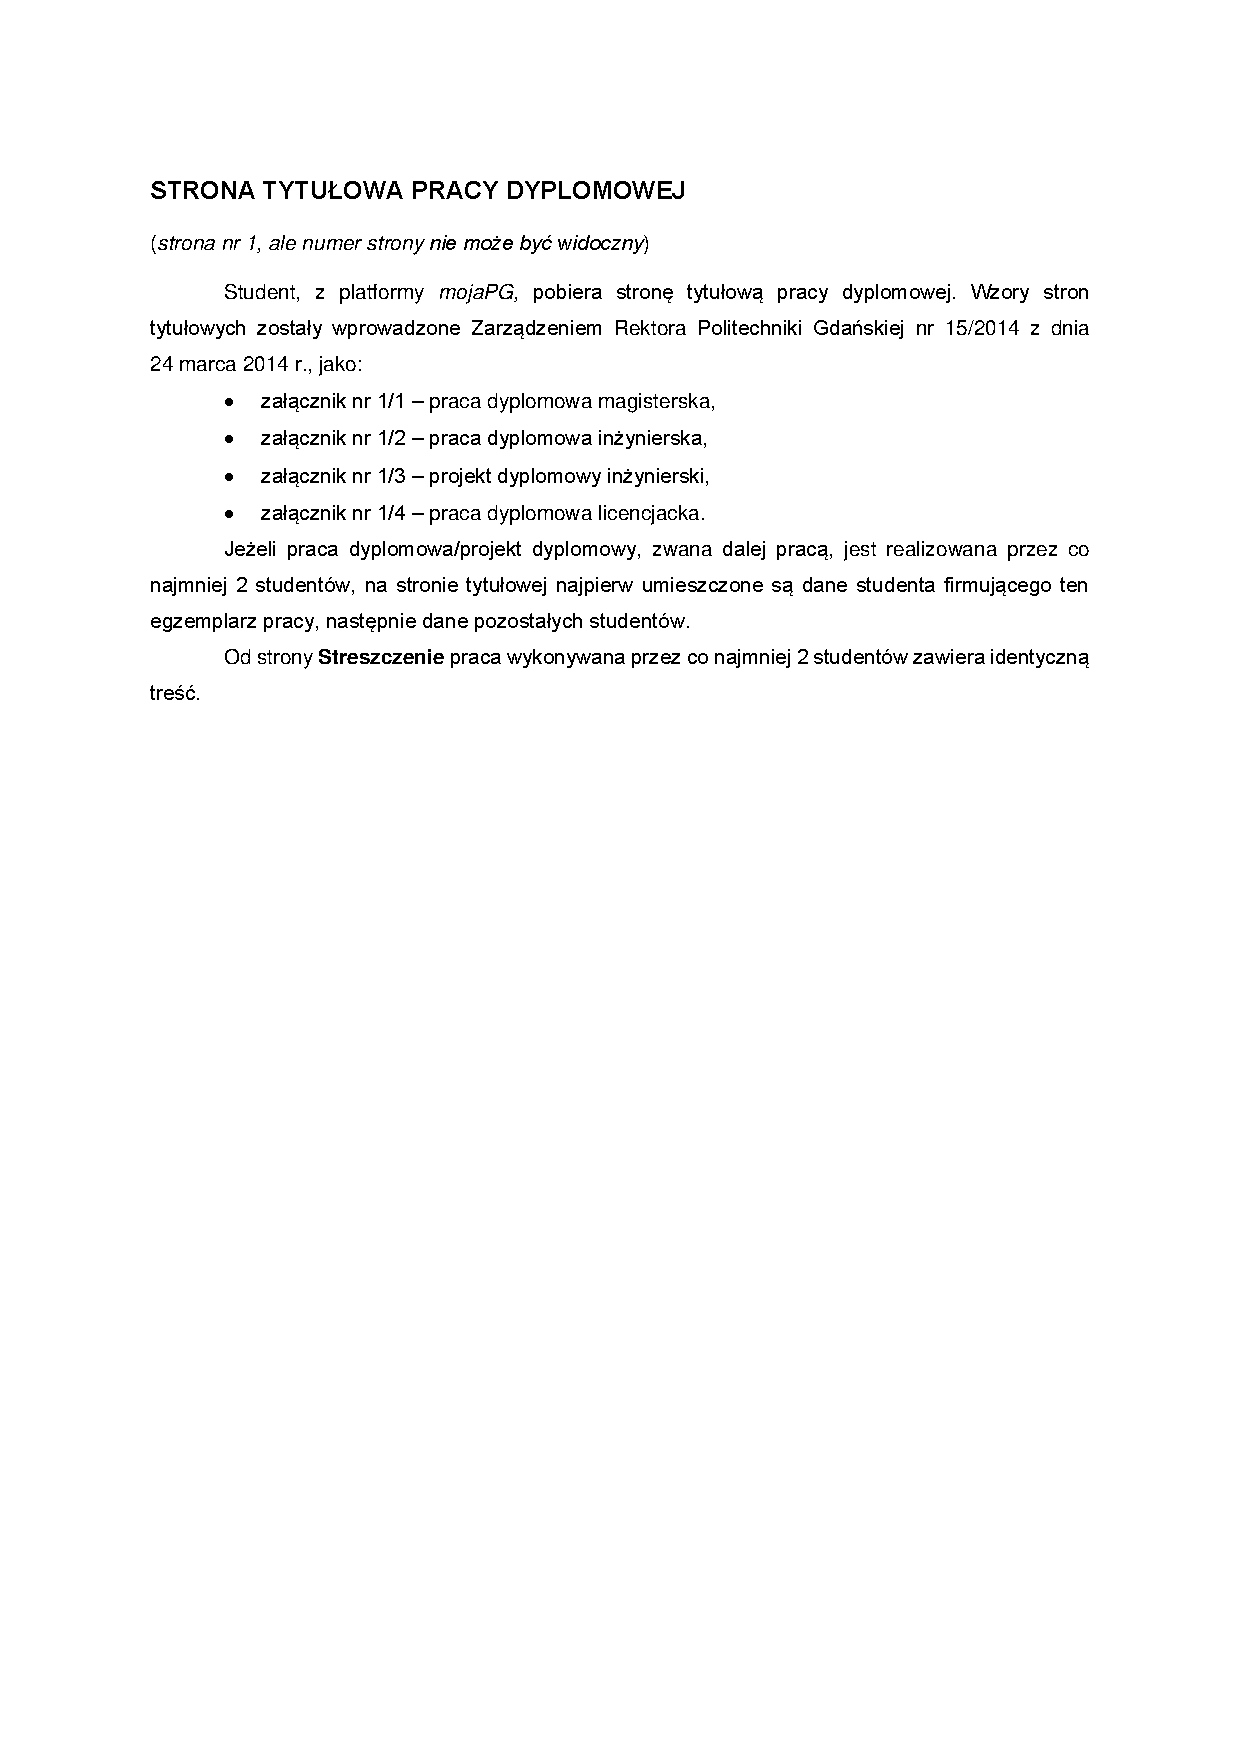
\includepdf{Chapters/Strona_tytulowa.pdf}
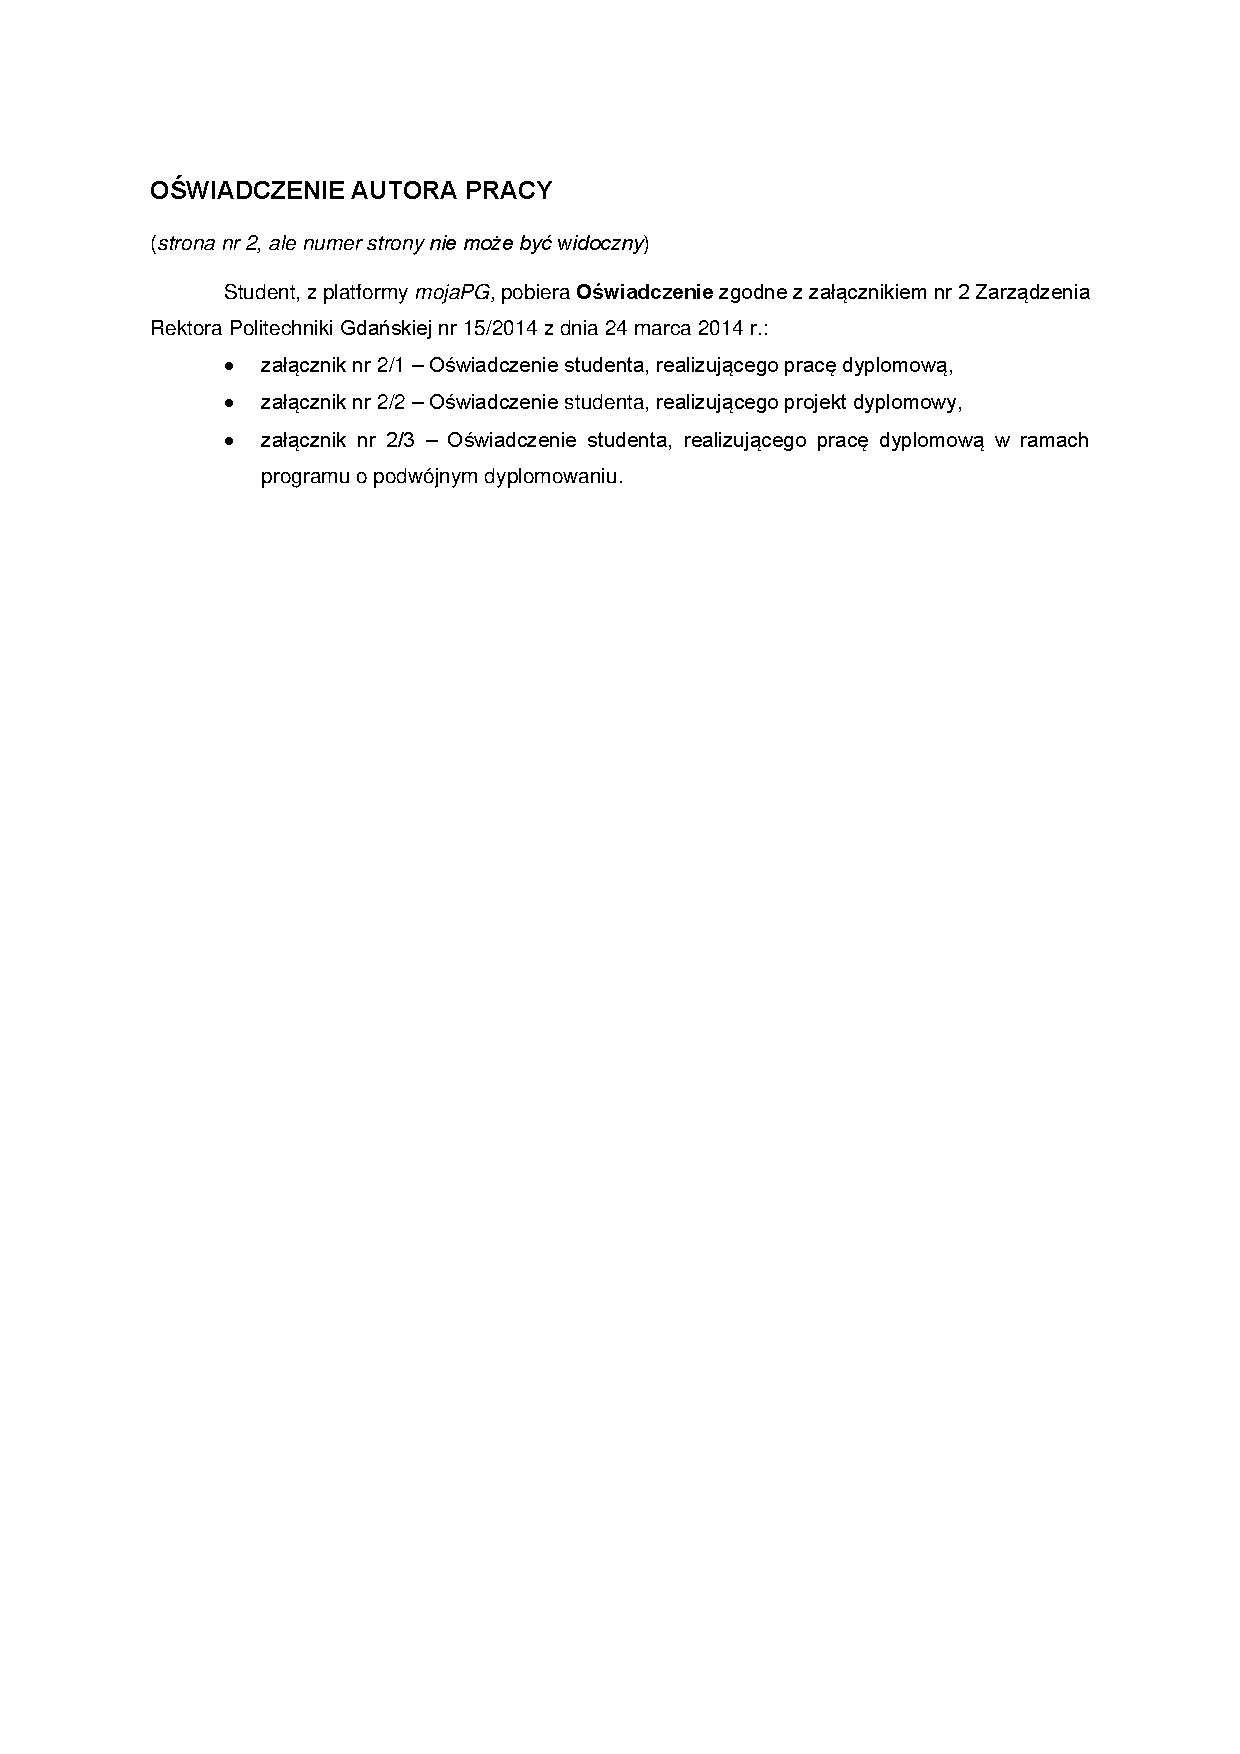
\includepdf{Chapters/Oswiadczenie.pdf}

% streszczenie PL, EN
\chapter*{Streszczenie}
\thispagestyle{plain}

(maksymalnie 1 strona, strona nr 3, numer widoczny)

Streszczenie powinno zawierać określenie problemu naukowego lub praktycznego do rozwiązania, cel i zakres pracy, zastosowane metody badań, wyniki i najważniejsze wnioski.

Jeżeli praca jest realizowana przez co najmniej 2 studentów, to w Streszczeniu należy określić indywidualny udział każdego studenta w realizowanej pracy, podając jakie zagadnienia przez każdego ze studentów zostały opracowane i wykonane. Należy również zamieścić informację jakie rozdziały lub podrozdziały dany student opracował (patrz Spis treści). Należy przyjąć, że punkty podrozdziałów muszą być opracowywane przez studenta odpowiedzialnego za realizację podrozdziału. Przykładowo, jeżeli praca jest realizowana przez studenta A i studenta B, to można przytoczyć zapis: imię i nazwisko studenta A – udział w rozdziałach 1, 7 oraz indywidualnie rozdział 2 oraz podrozdziały 3.1 i 4.2, itd., imię i nazwisko studenta B – udział w rozdziałach 1, 7 oraz indywidualnie rozdział 5 i 6 oraz podrozdziały 3.2 i 4.1, itd.

Celem pracy było wytworzenie aplikacji wspomagającej planowanie i realizację zadań, która wykorzystuje metodologię Geting Things Done autorstwa Davida Allena. Aplikacja ta powinna działać w rozproszonej architekturze w oparciu o łańcuch bloków (ang. Blockchain). 
\\\\
Słowa kluczowe: Blockchain, zdecentralizowany, planowanie
\\\\
Dziedzina nauki i techniki, zgodnie z wymogami OECD: . Nauki inżynieryjne i techniczne, Sprzęt komputerowy i architektura komputerów

\chapter*{Abstract}

The goal of the project was to create a system that supports task planning and execution, as well as enabling text communication between users. The task planning and execution support part was developed based on the Getting Things Done methodology by David Allen.

The main premise of the application was decentralization, so communication was implemented using a distributed architecture based on a Peer-to-Peer network. Data is stored using blockchain technology. Consensus is achieved through the proof of stake algorithm.

These solutions enhance the application's security because they significantly complicate data eavesdropping, impersonation, or manipulation of existing data. They also reduce the risk of data loss as there are multiple storage units. Data is transmitted via the HTTP protocol. It is also encrypted and electronically signed, which further increases security.

The application's interface was written in the QT framework, while the business logic was implemented in Python.
\\\\
Keywords: Blockchain, decentralization, planning, security

% spis treści
\tableofcontents

% wykaz skrótów
\chapter*{Wykaz ważniejszych oznaczeń i skrótów}
\addcontentsline{toc}{chapter}{Wykaz ważniejszych oznaczeń i skrótów}

% otoczenie abbrev zdefiniowane w macra.sty
\begin{abbrev}
\item[Klient] Instancja programu obsługiwana przez danego użytkownika
\item[P2P] Sieć typu peer-to-peer (równy z równym)
\item[IDE] Integrated Development Environment (Zintegrowane Środowisko Programistyczne)
\item[HTTP] Hypertext Transfer Protocol (Protokół Transmisji Hipertekstu)
\item[HTML] HyperText Markup Language (Hipertekstowy Język Znaczników)
\item[CSS] Cascading Style Sheets (Kaskadowe Arkusze Stylów)
\item[UTF-8] 8-bit Unicode Transformation Format (8-bitowy Format Transformacji Unicode)
\item[Backend] Warstwa przechowywania danych i logiki biznesowej
\item[ASCII] American Standard Code for Information Interchange (Amerykański Standardowy Kod Wymiany Informacji)
\item [SHA-256] 256-bit Secure Hash Algorithm (256-bitowy Bezpieczny Algorytm Haszujący)
\item[IEEE] Institute of Electrical and Electronics Engineers (Instytut Inżynierów Elektryków i Elektroników)
\item[IPFS] InterPlanetary File System (Międzyplanetarny System Plików)
\item[RSA] Algorytm Rivesta-Shamira-Adlemana
\item[AES] Advanced Encryption Standard (Zaawansowany Standard Szyfrowania)
\item[DES] Data Encryption Standard (Standard Szyfrowania Danych)
\item[PoS] Proof of Stake (Dowód Stawki)
\item[PoW] Proof of Work (Dowód Pracy)
\item[DPoS] Delegated Proof of Stake (Delegowany Dowód Stawki)
\item[PoC] Proof Of Capacity (Dowód Pojemności)
\item[GTD] Getting Things Done (Załatwianie Spraw)
\item[NIST] National Institute of Standards and Technology (Narodowy Instytut Norm i Technologii)
\item[RC6] Rivest cipher 6 (Szyfr Rivesta 6)
\item[MARS] Multiplication, Addition, Rotation, and Substitution  (Mnożenie, dodawanie, obrót i podstawianie)
\item[TLS] Transport Layer Security (Bezpieczeństwo Warstwy Transportowej)
\item[IPsec] Internet Protocol Security (Bezpieczeństwo Protokołu Internetowego)
\item[WPA] Wi-Fi Protected Access (Dostęp Chroniony Wi-Fi)
\item[ECB] Electronic Code Book (Tryb Elektronicznej Książki Kodowej)
\item[CBC] Cipher Block Chaining (Tryb Wiązania Bloków Zaszyfrowanych)
\item[CFB] Cipher Feedback (Tryb Sprzężenia Zwrotnego Szyfrogramu)
\item[OFB] Output Feedback (Tryb Sprzężenia Zwrotnego Wyjścia)
\end{abbrev}



% rozdziały i podrozdziały numerowane
\chapter{Wstęp i cel pracy}
\label{chap:wstep}
\textit{Autorzy: Maksym Nowak, Piotr Noga}
\par Celem naszej pracy jest wytworzenie aplikacji, która będzie wspomagać użytkowników programu w planowaniu oraz realizacji zadań przy wykorzystaniu metodologii Getting Things Done (GTD), opracowanej przez Davida Allena w jego książce o tym samym tytule \cite{GTD}. GTD to sposób odpowiedniego uporządkowywania planów i zadań tak, aby osoba mogła się skupić na ich realizacji, aniżeli na ciągłym myśleniu o nich \cite{DAllInt}. Jednym z głównych założeń naszego programu jest jego decentralizacja działania, tj. żaden klient nie pełni równocześnie funkcji centralnego serwera, przez który przepływają informacje do innych klientów. Każdy klient łączy się bezpośrednio z pozostałymi, którzy są połączeni ze sobą w sieci typu peer-to-peer (P2P). Z tym sposobem komunikacji klientów związany jest również sposób przechowywania danych, przekazywanych między nimi, gdyż w tym celu zostanie wykorzystana struktura danych zwana łańcuchem bloków (ang. Blockchain).

\section{Uzasadnienie potrzeby realizacji tematu}
Obecnie nie stanowi problemu znalezienie odpowiadającgo użytkownikowi narzędzia do planowania i realizacji zadań w oparciu o metodologię GTD \cite{GTD-apps}. Przykładami takich programów są m.in.:
\begin{itemize}
    \item Nirvana,
    \item Evernote,
    \item ClickUp,
    \item ToodleDo.
\end{itemize}
Programy te jednak mają jedną zasadniczą wadę, które zmotywowały nasz zespół do realizacji tego tematu: żadne z nich nie oferuje możliwości pracy w sposób zdecentralizowany. Mogą one działać jedynie na dwa sposoby:
\begin{itemize}
    \item korzystając z centralnego serwera,
    \item lokalnie.
\end{itemize}
Korzystanie z centralnego serwera oznacza, że użytkownik musi przesyłać dane na serwer firmy zarządzającej danym programem, co może wiązać się z naruszeniem jego prywatności, gdyż wgląd do danych mogą mieć również nieupoważnione osoby. Aplikacje działające lokalnie natomiast mają ograniczenie w postaci możliwości korzystania z nich tylko przez danego użytkownika w odrębie jednego urządzenia, zatem nie ma on możliwości udostępnienia swoich planów czy zadań z innymi upoważnionymi osobami.
\par Bliźniaczo podobna sytuacja ma się z aplikacjami zdecentralizowanymi. Tutaj również można znaleźć pełno rozwiązań spełniających to założenie, lecz żadne z nich nie implementuje w znacznym stopniu GTD. Można zatem stwierdzić, że w momencie redagowania niniejszej pracy dyplomowej, nie istnieje żadne takie rozwiązanie publicznie dostępne, które spełniałoby w pełni nasze wymagania.

\section{Podział prac}
W naszej pracy dyplomowej można wyodrębnić zadania poszczególnych członków w następujący sposób:
\begin{itemize}
    \item Bartosz Kołakowski:
        \begin{itemize}
            \item Lider grupy, odpowiedzialny za koordynowanie pracy i przydzielanie zadań całemu zespołowi. Zrealizował moduł szyfrowania i deszyfrowania wykorzysywany w logice biznesowej naszego programu. Zaimplementował również uzyskiwanie konsensusu PoS. Zmodyfikował w znacznym stopniu działanie mechanizmów związanych z Blockchainem 
        \end{itemize}
    \item Piotr Noga:
        \begin{itemize}
            \item Zrealizował pozostałe komponenty logiki biznesowej programu oraz połączenie jej z interfejsem graficznym.  
        \end{itemize}
    \item Michał Mróz:
        \begin{itemize}
            \item Zrealizował projektowanie i implementację wyglądu aplikacji oraz połączenie interfejsu graficznego z częścią logiki biznesowej aplikacji.  
        \end{itemize}
    \item Maksym Nowak:
        \begin{itemize}
            \item Zrealizował implementację interfejsu graficznego.  
        \end{itemize}
\end{itemize}
\chapter{Stan wiedzy}
\label{chap:stan_wiedzy}
\textit{Autor: Piotr Noga}
\par Zanim podjęliśmy się naszej pracy dyplomowej, przejrzeliśmy artykuły naukowe, literaturę oraz dostępne w Internecie implementacje projektów związanych z naszym tematem pracy. Mogliśmy w ten sposób ugruntować swój stan wiedzy.
\section{Artykuły naukowe}
\label{sec:ArtykulyNaukowe}
Zacznijmy od przeglądu artykułów naukowych. Skupiliśmy swoją uwagę głównie na artykuły naukowe napisane w języku angielskim, lecz staraliśmy się znaleźć również publikacje polskojęzyczne. W poszukiwaniu odpowiednich artykułów naukowych skorzystaliśmy z udostępnianego przez Bibliotekę Politechniki Gdańskiej dostępu do zagranicznych bibliotek cyfrowych. Tymi bibliotekami, z których głównie korzystaliśmy, były:
\begin{itemize}
    \item IEEE Xplore
    \item ACM Digital Library
    \item Springer
    \item Scopus | Elsevier
\end{itemize}
Korzystaliśmy również z ogólnodostępnych bibliotek cyfrowych oraz wydawnictw, oferujących artykuły napisane w języku polskim, takich jak:
\begin{itemize}
    \item Google Scholar
    \item Polska Bibliografia Naukowa
    \item MDPI
\end{itemize}
Swoje poszukiwania rozpoczęliśmy od sprawdzenia, czy istnieją artykuły naukowe odnoszące się w całości do naszego tematu pracy. Mimo próby znalezienia odpowiednich artykułów  poprzez używanie różnych fraz kluczowych w języku polskim, jak również w angielskim, takich jak: "\textbf{system} \ang{system}, \textbf{dispersion} \ang{support}, \textbf{planowanie} \ang{planning}, \textbf{zdecentralizowany} \ang{decentralized}, \textbf{aplikacja} \ang{application}, \textbf{poufność} \ang{confidentiality}, \textbf{niezaprzeczalność} \ang{non-repudiation}, \textbf{rozproszenie} \ang{distributed}, \textbf{konsensus} \ang{consensus}, \textbf{łańcuch bloków} \ang{blockchain}, GTD (skrót od Getting Things Done)", w żadnej z bibliotek nie ma ani jednego artykułu naukowego, który wprost omawiałby aplikację, która implementuje wszystkie założenia naszego systemu. Można znaleźć artykuły odnoszące się jedynie do wybranych zagadnień. Wśród nich można wyróżnić prezentacje implementacji aplikacji zdecentralizowanych. Natrafiliśmy również na jeden z takich artykułów \cite{EvolutionOfBlockchainCon}, który zdecydowanie wpłynął na nasz wybór algorytmu uzgadniania konsensusu łańcuchów bloków, gdyż w szczegółowy sposób omówił każdy z nich, porównał je między sobą, wypisując ich wady i zalety oraz zawierał od razu odnośniki również do innych prac naukowych, w których zostały omówione poszczególne algorytmy.

\section{Literatura}
\label{sec:Literatura}
W przypadku literatury sprawa wygląda podobnie co przy artykułach naukowych. Nie ma takich publikacji, które łączyłyby większość zagadnień związanych z naszą pracą dyplomową, a co najwyżej tylko kilka z nich. Nie mniej jednak można przebierać w wielu książkach związanych z łańcuchem bloków takich jak chociażby "Mastering Blockchain" \cite{MasteringBlockchain}, "Blockchain, Crypto and DeFi" \cite{BCDF}, "Build Your Own Blockchain" \cite{BuildBlockchain} czy też "Bubble Or Revolution?" \cite{BubbleOrRevolution}, które często tłumaczą to zagadnienie w mniej bądź bardziej techniczny sposób, lecz z pewnością w wystarczającym dla nas w zupełności, co z pewnością przyłożyło się na zastosowanie tej struktury danych. Nieodzowną pomocą w naszej pracy okazała się także książka autorstwa Davida Allena pt. "Getting Things Done" \cite{GTD}, która w kompleksowy sposób wyjaśniła nam zasady stojące za tytułową metodologią, którą wdrożyliśmy w naszej aplikacji. Jeśli chodzi o wiedzę kryptograficzną to korzystaliśmy z książek "Kryptografia: w teorii i w praktyce" \cite{KryptografiaWTeoriiPraktyce}, "Kryptografia i ochrona danych" \cite{KryptografiaOchronaDanych} i "Algorytmy kryptograficzne" \cite{AlgorytmyKryptograficzne}. Książki przedstawiające tematykę kryptowalut i zawartych w nich mechanizmów to między innymi "Blockchain. Przewodnik po łańcuchu bloków." \cite{BlockchainPrzewodnikPoLanuchu}, "Blockchain. Fundament nowej gospodarki" \cite{BlockchainFundamentGospodarki} i "Dowód stawki" \cite{DowodStawki}. O aplikacjach zdecentralizowanych i kominukacji równy z równym (peer-to-peer) dowiedzieliśmy się z książek "Projektowanie systemów rozproszonych" \cite{ProjektowanieSystemowRozproszonych} i "Peer-to-Peer. Harnessing the Power of Disruptive Technologies" \cite{PeerToPeer}. Wiedzę o tworzeniu aplikacji internetowych (głownie za pomocą platformy programistycznej Flask) uzyskaliśmy z "Flask. Tworzenie aplikacji internetowych w Pythonie" \cite{FlaskTworzenieAplikacji}, "Mastering Flask" \cite{MasteringFlask} i "Flask By Example" \cite{FlaskExample}. Przy tworzeniu graficznego interfejsu użytkownika (GUI) korzystaliśmy z takich źródeł - "Tkinter GUI Application Development Cookbook" \cite{TkinterCookbook}, "Biblioteki Qt. Zaawansowane programowanie przy użyciu C++" \cite{BibliotekiQt} i "Qt5 Python GUI Programming Cookbook" \cite{QTPython}. %TODO: Również przydatnym zasobem wiedzy były książki zahaczające o tematykę aplikacji zdecentralizowanych.


\section{Projekty użytkowników}
\label{sec:ProjektyUzytkownikow}
Wśród innych entuzjastów technologii, którzy dzielą się z innymi swoimi projektami, znaleźć można różnorakie programy, które w mniejszym lub większym stopniu spełniają założone przez nas cele pracy dyplomowej. Jednymi z najbliższych naszemu programowi są implementacje programów zdecentralizowanych, które posiadają wbudowany moduł planowania zadań, bądź moduł czatu. Przykładami takich programów są "ToDo-DApp" \cite{ToDo_DApp} i "DAPP-todo" \cite{DAPP_todo} w przypadku modułu planera oraz odnośnie modułu czatu "chatDapp" \cite{chatDapp} i "dappchat" \cite{dappchat}. Inną przydatną implementacją był "BlockChat" \cite{blockchat}, w którym była możliwość wysyłania wiadomości przez sieć, a następnie tworzenie z nich bloków opartych na dowodzie pracy jako algorytmie osiągania konsensusu. Inną implemntacją opartą o architekturę rozproszoną i blockchain jest \cite{PythonBlockchain}. To tylko kilka z przykładowych projektów, gdyż nie sposób jest ich zliczyć, lecz wszystkie z nich, jakie przejrzeliśmy, nie łączyły ze sobą obu tych części ze sobą.%TODO

\section{Rozwiązania komercyjne}
\label{sec:RozwiazaniaKomercyjne}
By dopełnić swój stan wiedzy, przejrzeliśmy również jakie są dostępne obecnie na rynku komercyjne rozwiązania, które spełniają jedne z naszych celów. Warto wspomnieć, o platformie zrealizowanej ze środków publicznych (budżet około 5 milionów \cite{IDB})  "lubbezposrednio.pl" \cite{lubBezPosrednio}, która umożliwia głosowanie elektroniczne z wykorzystaniem technologii blockchain. Jednak, tak jak w poprzednich sekcjach nie da się znaleźć żadnego takiego produktu, który umożliwiałby wspomaganie planowania zadań i ich realizacji, który działałby w sposób zdecentralizowany oraz rozproszony. %TODO 

\section{Podsumowanie stanu wiedzy}
\label{sec:PodsumowanieWiedzy}
Podsumowując wszystkie zabrane informacje o obecnym stanie wiedzy, nasuwa się następująca myśl - obecnie nie ma rozwiązania które spełniałoby wszystkie porządane cechy - wspomaganie planowania zadań i ich realizacji, umożliwienie pracy w sposób zdecentralizowany, działanie w architekturze rozproszonej, korzystanie z algorytmu osiągania konsensusu i zapewnienie poufności wiadomości użytkowników. Nasza praca dyplomowa ma na celu między innymi zmianę tego stanu rzeczy i wypuszczenie na świat pierwszego produktu w takim stylu.
\chapter{Wykorzystane algorytmy i ich charakterystyka}
\textit{Autor: Bartosz Kołakowski}
\setlength{\parindent}{0pt}

\section{Szyfrowanie symetryczne}
\subsection{Opis szyfrowania symetrycznego}
Szyfrowanie symetryczne (inaczej szyfrowani z kluczem tajnym czy szyfrowanie z kluczem pojedynczym) jest rodzajem szyfrowania, gdzie do operacji szyfrowania jak i deszyfrowania wykorzystywany jest tylko jeden klucz. W przeciwieństwie do klucza publicznego w szyfrowaniu asymetrycznym klucz w szyfrowaniu symetrycznym jest tajny i nie powinien być nikomu ujawniany. Istnieje wiele algorytmów szyfrowania symetrycznego, są to na przykład Twofish, Serpent czy AES. W tej implementacji został wybrany AES, który jest jednym z najczęściej używanych algorytmów klucza pojedynczego. Jego zaletami jest bezpieczeństwo i odporności na złamanie szyfru, o których zostanie napisane w dalszej części pracy. Inną cechą tego algorytmu jest jego wydajność, w porównaniu do innych algorytmów szyfrowania symetrycznego (w porównaniu do algorytmów szyfrowania asymetrycznego oczywiście też, ale kryptografia klucza publicznego jest kilka rzędów wolniejsza od kryptografii z jednym kluczem). Między innymi to wydajność AES (bezpieczeństwo oczywiście też) była cechą, która sprawiła, że został on wybrany nad algorytmami Serpent, Twofish, RC6 i MARS. Algorytmy te same w sobie również były bezpieczne, ale ich gorsza wydajność sprawiła, że to nie one zostały w 2001 wybrane przez National Institute of Standards and Technology na następcę DES. Inną ważną cechą AES jest jego powszechne stosowanie i popularność, jest on między innymi wykorzystywany w protokołach TLS (Transport Layer Security), IPsec (Internet Protocol Security) czy WPA (WiFi Protected Access).

Szyfrowanie symetryczne pokazane jest na rysunku \ref{fig:AES1}
\begin{figure}[H]
    \centering
    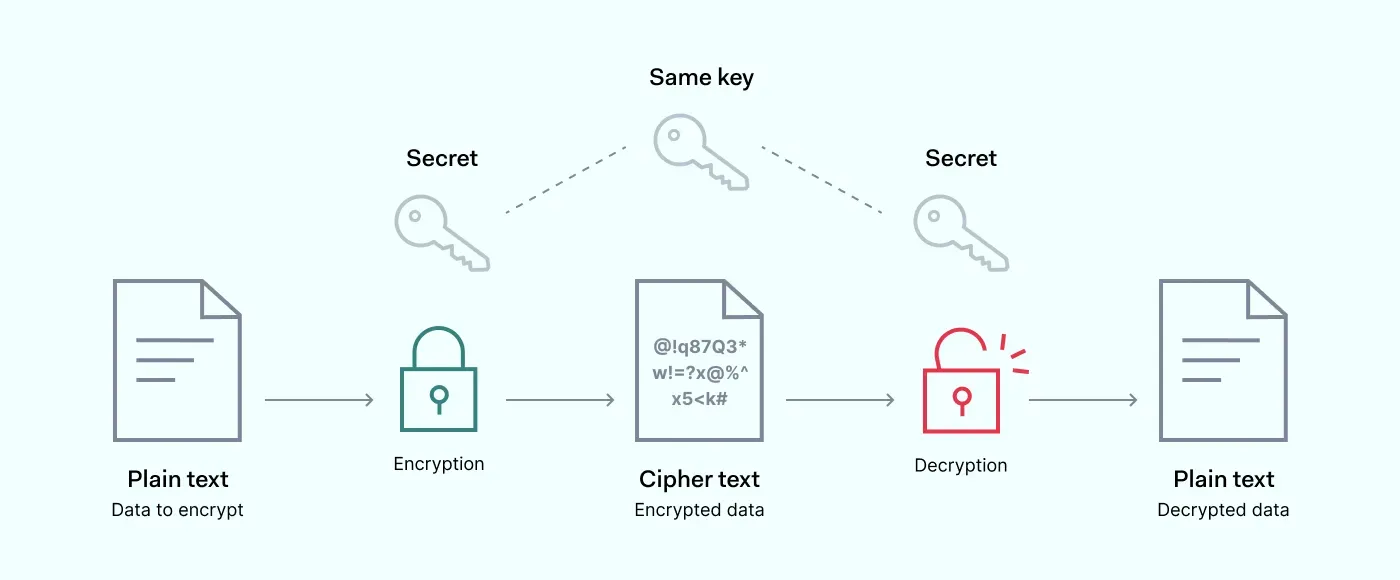
\includegraphics[width=\textwidth]{Images/AES1.png}
    \caption{Schemat szyfrowania symetrycznego}
    \label{fig:AES1}
\end{figure}

Algorytm AES (skrót od Advanced Encryption Standard) jest jednym z najbardziej znanych algorytmów kryptografii symetrycznej. Jego zdecydowaną zaletą jest fakt, że ten algorytm jest dobrze przetestowany i powszechnie używany. Jego historia opiera się na tym, że wcześniej powszechnie używany algorytm DES (Data Encryption Standard) nie zapewniał już odpowiedniego poziomu bezpieczeństwa, między innymi przez krótką długość klucza i małą długość bloku co powodowało niską odporność na ataki. W konkursie ogłoszonym przez NIST (skrót od National Institute of Standards and Technology) mającym zastąpić DES wygrał algorytm, którego oryginalna nazwa brzmiała Rijndael. Aby zrozumieć, dlaczego AES został wybrany i jest tak powszechnie stosowany zostanie przedstawione jak działa i zobaczyć jego charakterystyczne cechy.

\vspace{0.3\baselineskip}

Tak jak wcześniej wspomniano AES jest algorytmem szyfrowania symetrycznego, który opiera się na blokach. Mają one stały rozmiar 128 bitów. Cały algorytm opiera się na wielu matematycznych operacjach, które są podzielone na rundy. To, ile jest rund zależy od tego jaka jest długość (10 rund dla klucza 128-bitowego, 12 rund dla klucza 192-bitowego, 14 rund dla klucza 256-bitowego). Operacje są wykonywane na macierzach 4x4 bajty.

\vspace{0.3\baselineskip}

Operacje wykonywane w każdej z rund przedstawiają się następująco:
\begin{enumerate}
    \item Zamiana bajtów – zamiana każdego bajtu według schematu w tabeli podstawień, ma to na celu to, żeby te operacje były nieliniowe,
    \item Zamiana wierszy – przesunięcie określonej ilości wierszy macierzy, w celu dyfuzji danych
    \item Mieszanie kolumn – jest to osiągnę przez mnożenie elementów tych kolumn
    \item Dodanie klucza – do macierzy dodawany jest klucz rundowy (głównie przez wykorzystanie operacji alternatywy rozłącznej)
\end{enumerate}
Wszystkie te operacje mają na celu zaciemnienie oryginalnych danych tak, żeby nie dało się ich odszyfrować bez znajomości symetrycznego klucza, a fakt, że operacje są wykonywane w wielu rundach czyni algorytm jeszcze bardziej trudniejszym do złamania.

\vspace{0.3\baselineskip}

Jak wyglądają operacje w algorytmie AES pokazane jest na rysunku \ref{fig:AES2}
\begin{figure}[H]
    \centering
    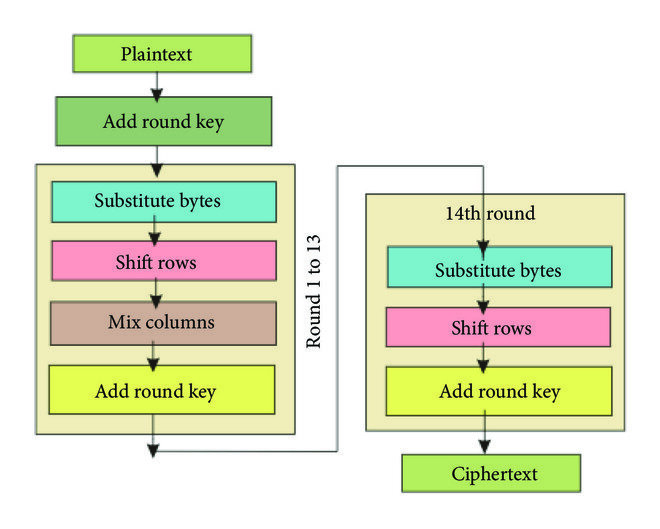
\includegraphics[width=\textwidth]{Images/AES2.jpg}
    \caption{Schemat działania AES}
    \label{fig:AES2}
\end{figure}

\subsection{Użycie szyfrowania symetrycznego w praktyce}

\begin{lstlisting}[caption={Szyfrowanie danych}]
def encrypt_data_ecb(data, key):
    cipher = AES.new(key, AES.MODE_ECB)
    encrypted_data = cipher.encrypt(pad(data.encode(), AES.block_size))
    encrypted_base64 = base64.b64encode(encrypted_data).decode('utf-8')
    return encrypted_base64
\end{lstlisting}
\listings{Szyfrowanie danych}
Szyfrowanie danych odbywa się przez funkcję, której parametrami są tekst podany do zaszyfrowania oraz klucz sesyjny. W samej funkcji najpierw tworzony jest obiekt szyfrujący AES, który jest ustawiony w trybie wiązania bloków zaszyfrowanych ECB - Electronic CodeBook (Tryb Elektronicznej Książki Kodowej). Dlaczego akurat w takim trybie, a nie na przykład CBC - Cipher Block Chaining (Tryb Wiązania Bloków Zaszyfrowanych), CFB - Cypher Feed Back (Tryb Sprzężenia Zwrotnego Szyfrogramu) czy OFB - Output Feedback (Tryb Sprzężenia Zwrotnego Wyjścia) - powodem jest charakterystyka tego trybu - pożądaną cechą w systemie jest to, aby był on deterministyczny, co wyklucza elementy losowe, a ECB jako jedyny z powszechnie używanych trybów wiązania bloków zaszyfrowanych nie korzysta z losowych wektorów inicjalizujących. Następnie szyfrujemy z wykorzystaniem wcześniej stworzonego obiektu szyfrującego, a wynik tej operacji przekonwertowujemy do łańcucha znaków za pomocą Base64.

\begin{lstlisting}[caption={Deszyfrowanie danych}]
def decrypt_data_ecb(encrypted_base64, key):
    encrypted_data = base64.b64decode(encrypted_base64)
    cipher = AES.new(key, AES.MODE_ECB)
    decrypted_data = unpad(cipher.decrypt(encrypted_data), AES.block_size)
    return decrypted_data.decode()
\end{lstlisting}
\listings{Deszyfrowanie danych}
W funkcji deszyfrującej najpierw zaszyfrowane dane są konwertowane z formatu Base64 na ciąg bajtów, potem podobnie jak w operacji szyfrowania tworzony jest nowy obiekt szyfrujący, którego tryb wiązania bloków zaszyfrowanych to ECB. Następnie deszyfrujemy dane za pomocą klucza sesyjnego i usuwamy zbędne wypełnienie.

\section{Szyfrowanie asymetryczne}

\subsection{Opis szyfrowania asymetycznego}
Szyfrowanie asymetryczne (inaczej nazywane szyfrowaniem klucza publicznego) to rodzaj szyfrowania, w którym występują dwa klucze – prywatny i publiczny. Klucz prywatny jest generowany na podstawie odpowiednio dużych liczb pierwszych i nie powinien być nikomu udostępniany. W kryptografii asymetrycznej klucz prywatny służy do odszyfrowywania. Drugim kluczem jest klucz publiczny, który jest generowany na podstawie klucza prywatnego i może on być udostępniany innym użytkownikom. Klucz publiczny w kryptografii klucza tajnego wykorzystywany jest przy szyfrowaniu. Jest wiele algorytmów kryptografii asymetrycznej – RSA, ElGamal czy Elliptic Curve Cryptography. W tej implementacji wykorzystano jeden z najczęściej wykorzystywanych algorytmów – jest to RSA. Algorytm RSA (jest to skrót od Rivest–Shamir–Adleman) jest jednym z najbardziej popularnych i najczęściej wykorzystywanych algorytmów kryptografii asymetrycznej. Jego istotnymi zaletami są bezpieczeństwo i wysoka odporność na ataki.

Zobrazowanie szyfrowania symetrycznego na grafice \ref{fig:RSA1}
\begin{figure}[H]
    \centering
    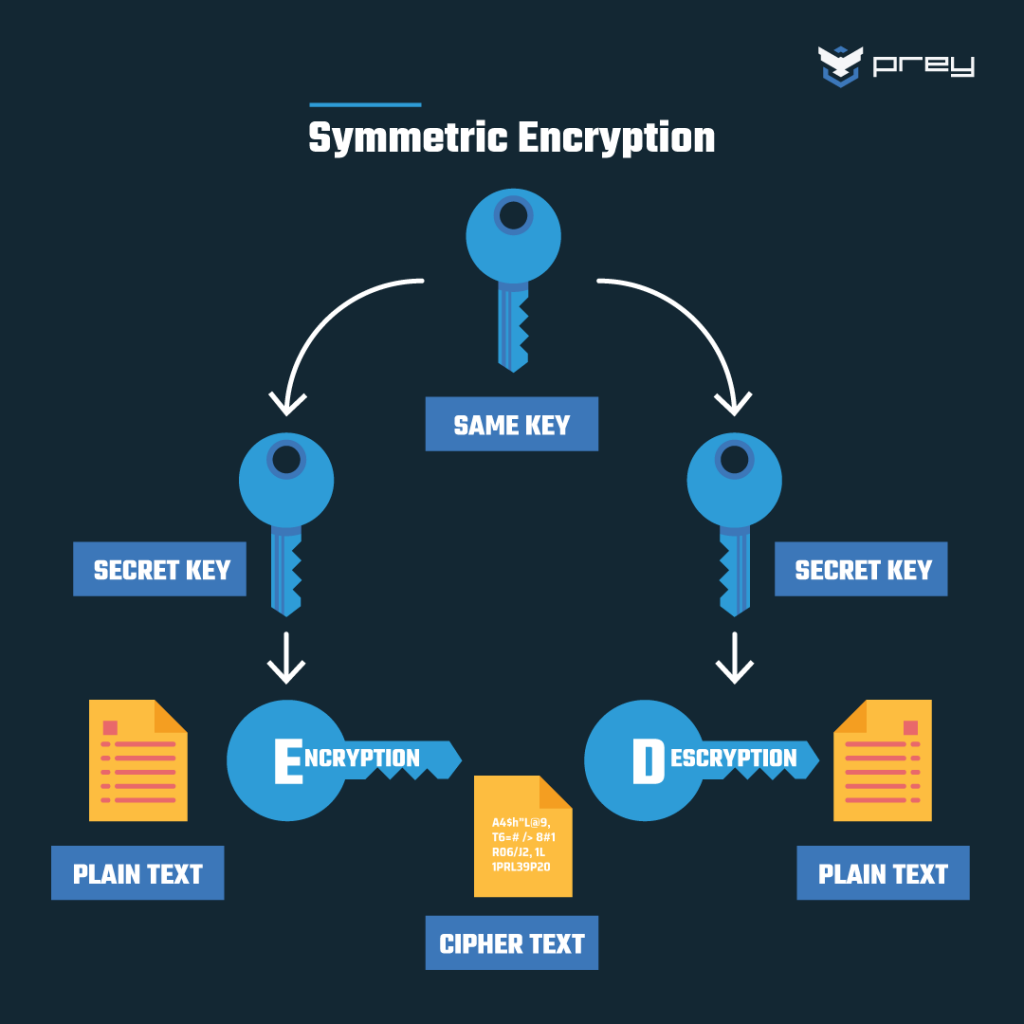
\includegraphics[width=\textwidth]{Images/RSA1.png}
    \caption{Schemat szyfrowania symetrycznego}
    \label{fig:RSA1}
\end{figure}

\vspace{0.3\baselineskip}

Szczegółowe działanie algorytmu RSA polega na tym, że wybiera się dwie duże liczby pierwsze, z których potem oblicza się moduł n i wartość z funkcji Eulera na podstawie tego modułu. Klucz publiczny jest liczbą względnie pierwszą do wartości funkcji Eulera. Klucz prywatny jest odwrotnością multiplikatywną wartości klucza publicznego modulo wartości funkcji Eulera. Szczegółowo przedstawia się to na wzorach:

Oznaczenie początkowych liczb - wzór \ref{eq:first}
\begin{equation}
    p, \; q-losowe, \; ogromne \; liczby \; pierwsze
    \label{eq:first}
\end{equation}
\equations{Oznaczenie początkowych liczb}
Wartość modułu - wzór \ref{eq:second}
\begin{equation}
    n=p*q
    \label{eq:second}
\end{equation}
\equations{Wartość modułu}
Wartość funkcji Eulera - wzór \ref{eq:third}
\begin{equation}
    \phi(n)=(p-1)*(q-1)
    \label{eq:third}
\end{equation}
\equations{Wartość funkcji Eulera}
Klucz publiczny - wzór \ref{eq:fourth}
\begin{equation}
    e \in \{NWD(\phi(n),e)=1, \; 1 \leqslant e \leqslant \phi(n)\}
    \label{eq:fourth}
\end{equation}
\equations{Klucz publiczny}
Klucz prywatny - wzór \ref{eq:fifth}
\begin{equation}
    d= e^{-1} (mod \; \phi(n))
    \label{eq:fifth}
\end{equation}
\equations{Klucz prywatny}
Szyfrowanie wiadomości odbywa się korzystając ze wzoru \ref{eq:sixth}
\begin{equation}
    C= M^e, \; C-zaszyfrowana \;  wiadomość, \; M-oryginalny \; tekst, \; e-klucz \; publiczny
    \label{eq:sixth}
\end{equation}
\equations{Szyfrowanie wiadomości}
Deszyfrowanie odbywa się za pomocą wzoru \ref{eq:seventh}
\begin{equation}
    M= C^d, \; M-deszyfrowana \; wiadmość, \;C-zakodowany \; tekst, \; d-klucz \; prywatny
    \label{eq:seventh}
\end{equation}
\equations{Deszyfrowanie wiadomości}
Bezpieczeństwo tego algorytmu opiera się na tym, że odwrócenie tych operacji i uzyskanie klucza prywatnego na podstawie czyjegoś klucza publicznego oraz treści zaszyfrowany i deszyfrowanych wiadomości jest obliczeniowo bardzo trudne.

Ukazanie RSA w skomplikowanych systemach na rysunku \ref{fig:RSASieci}
\begin{figure}[H]
    \centering
    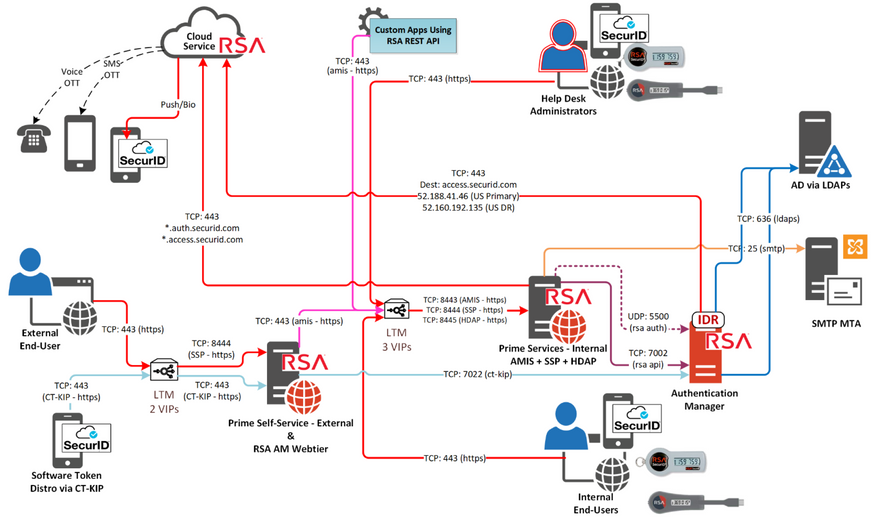
\includegraphics[width=\textwidth]{Images/RSASieci.png}
    \caption{Pokazanie RSA w zaawansowanych systemach}
    \label{fig:RSASieci}
\end{figure}

\subsection{Użycie szyfrowania asymetrycznego w praktyce}
\begin{lstlisting}[caption={Generowanie klucza prywatnego}]
self.private_key = rsa.generate_private_key(
            public_exponent=65537,
            key_size=2048,
            backend=default_backend()
)
\end{lstlisting}
\listings{Generowanie klucza prywatnego}

Każdy z użytkowników posiada wygenerowany klucz prywatny, jest on generowany losowo i niezależnie od innych. Inni użytkownicy nie wiedzą jaki jest klucz prywatny danego użytkownika. W stosowanej przez implementacji wykładnik publiczny ma zalecaną wartość dosyć małej liczby pierwszej (65537), a długość klucza to 2024 bitów, co sprawia, że algorytm jest wydajniejszy (to pokazuje różnicę między kryptografią asymetryczną, a kryptografią jednego klucza, gdzie jego długość w standardowych formatach AES to co najwyżej 256 bitów).


\begin{lstlisting}[caption={Generowanie klucza publicznego}]
self.public_key = self.private_key.public_key()
\end{lstlisting}
\listings{Generowanie klucza publicznego}

Klucz publiczny jest generowany na podstawie klucza publicznego, gdyż w kryptografii asymetrycznej klucze są między sobą powiązane.
\begin{figure}[H]
    \centering
    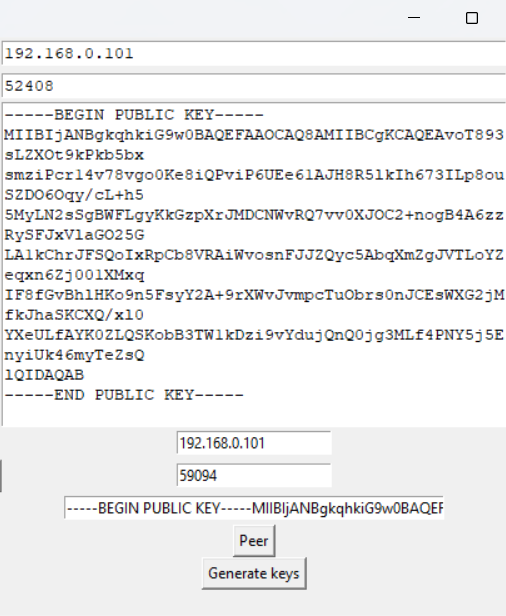
\includegraphics[width=\textwidth]{Images/CodeX13.png}
\end{figure}
Aby skutecznie połączyć się i komunikować się z innym użytkownikiem potrzebna jest znajomość jego klucza publicznego, dlatego w implementacji systemu przy nawiązywaniu połączenia podawany jest klucz publiczny (z którym nie ma żadnego zagrożenia bezpieczeństwa, aby został upubliczniony dla innych, w przeciwieństwie do klucza prywatnego).

\vspace{0.3\baselineskip}

W implementacji systemu pojawił się następującym problemem, mianowicie pożądane jest, aby wiadomości wysyłane przez sieć były łatwo dostępne dla innych użytkowników, którzy są członkami sieci, ale żeby ich treść nie była dostępna dla osób z zewnątrz (nie można ich przesyłać przez sieć jako zwykły tekst, ponieważ wtedy istniałaby możliwość podsłuchania i zostałby zaburzony jeden z filarów naszego systemu, czyli poufność wiadomości). Z tego powodu szyfrowanie wiadomości odbywa się w sposób symetryczny. Jednakże teraz może pojawić się pytanie czym będzie klucz w szyfrowaniu z pojedynczym kluczem i jak go ustalić w sposób bezpieczny. Tu jako rozwiązaniem jest szyfrowanie asymetryczne.

Każdy z użytkowników generuje losowy klucz sesyjny i w momencie powiększania się grupy (dodania nowego użytkownika) lub jej się zmniejszenia (usunięcie jednego z użytkowników) klucz sesyjny generuje się na nowo. Potem jeden z użytkowników jest w momencie zmiany składu grupy wybierany jako osoba mająca rozesłać klucz sesyjny.


\begin{lstlisting}[caption={Wybieranie osoby mającej rozesłać klucz sesyjny}]
def drawPerson(self):
    keyList = []
    for peer in self.peers:
        addrPort = {"addr": peer.addr, "port": peer.port}
        keyList.append(addrPort)
    myAddrPort = {"addr": ip(), "port": self.port}
    keyList.append(myAddrPort)
    sortedAddrPortList = sorted(keyList, key=lambda x: x["port"])
    keyRaw = " ".join(str(x["port"]) for x in keyList)
    self.drawString = keyRaw
    numeric_seed = int.from_bytes(hashlib.
    sha256(keyRaw.encode('utf-8')).digest())
    random.seed(numeric_seed)
    chosen_addr_port = random.choice(sortedAddrPortList)
    return chosen_addr_port
\end{lstlisting}
\listings{Wybieranie osoby mającej rozesłać klucz sesyjny}

Tak samo jak w przypadku Dowodu Stawki mechanizm losowania osoby mającej wysyłać klucz sesyjnym innym musi być taka sama dla wszystkich, tak oby osoba wysyłająca była w każdej instancji programu taka sama, inaczej użytkownicy mieliby różne klucze sesyjne co uniemożliwiłoby komunikację. Tworzy się lista użytkowników, którą następnie jest sortowana, aby każdy program miał ją w takiej samej postaci. Potem lista zamieniana jest na łańcuch znaków i używając deterministycznej funkcji skrótu (zwracającej te same wyniki dla tych samych danych) hashlib.sha256 (a nie na przykład domyślnej funkcji hash() w Pythonie, która nie jest deterministyczna) uzyskiwana jest wartość, która będzie ziarnem dla generatora liczb losowych i następnie wylosowany przez ten generator użytkownik (za pomocą standardowej funkcji random.choice()) będzie taki sam we wszystkich instancjach programu.

\begin{lstlisting}[caption={Uaklualnienie klucza sesyjnego}]
def update_group_session_key(self):
    self.EncryptedKBytes = encrypt_with_public_key
    (self.public_key, self.random_key)
    self.EncryptedKString = base64.b64encode(self.
    EncryptedKBytes).decode('utf-8')
    for peer in self.peers:
        peer.EncryptedKBytes = encrypt_with_public_key
        (peer.PKBytes, self.random_key)
        self.EncryptedKString = base64.b64encode
        (peer.EncryptedKBytes).decode('utf-8')
\end{lstlisting}
\listings{Uaklualnienie klucza sesyjnego}
Następnie po wylosowaniu osoby będącej odpowiedzialną za wysyłanie klucza ta osoba rozsyła do siebie klucz sesyjny zaszyfrowany swoim własnym kluczem publicznym, a do innych osób w sieci (biorąc pod uwagę niezmiennik, że każdy z każdym w danej grupie jest połączony) rozsyła klucz sesyjny zaszyfrowany kluczem publicznym danej osoby (właśnie dlatego, przy nawiązywaniu połączenia klucz podawany jest klucz publiczny – inaczej nie dało by się przekazać innym klucza sesyjnego z zachowaniem poufności). Dodatkową informacją godną uwagi jest fakt, że przy wysyłaniu innym zakodowanego klucza sesyjnego jest on poprzedzany nagłówkiem w celu łatwiejszego odebrania przez adresatów wiadomości.

\begin{lstlisting}[caption={Deszyfrowanie klucza sesyjnego}]
def convert_key(base64keyEncypted):
    byteKey = base64.b64decode(base64keyEncypted)
    decryptedSessionKey = me.private_key.decrypt(
        byteKey,
        padding.OAEP(
            mgf=padding.MGF1(algorithm=hashes.SHA256()),
            algorithm=hashes.SHA256(),
            label=None
        ))
    return decryptedSessionKey
\end{lstlisting}
\listings{Deszyfrowanie klucza sesyjnego}
Każdy z odbiorców po otrzymaniu klucza sesyjnego zakodowanego przez klucz publiczny w formacie Base64, korzysta z funkcji konwertującej,.pierwszą operacją jest zamienienie z typu łańcuchu znaków na format ciągu bajtów. Potem przebiega typowa dla kryptografii asymetrycznej operacja deszyfrowania kluczem prywatnym danego użytkownika, jednak szczególnie ważnym w niej jest fakt, że jest ona deterministyczna dla tych samych danych wejściowych do odszyfrowania, co oznacza, że jeśli podamy klucz sesyjny zaszyfrowany kluczem publicznym danego użytkownika i odszyfrujemy go jego kluczem prywatnym to zawsze wyjdzie nam poprawny klucz sesyjny z początku procesu. Ten klucz będzie potem wykorzystywany do odszyfrowania pojedynczych wiadomości w bloku przy wykorzystywaniu kryptografii klucza tajnego.

\section{Algorytmy osiągania konsensusu}
W kryptowalutach stosuje się wiele metod konsensusu z czego najbardziej popularne z nich to Dowód Pracy i Dowód Stawki, ale inne również znane to Dowód Pojemności i Delegowany Dowód Stawki. Aby uzasadnić która z nich została zastosowana w implementacji systemu, warto przeanalizować wszystkie z nich i zobaczyć ich wady i zalety.
\subsection{Dowód Pracy}
Dowód Pracy (angielski - Proof of Work) jest jedną z najstarszych metod konsensusu stosowanych w kryptowalutach gdzie dla każdego bloku wiadomości przypisana jest określona funkcja skrótu i użytkownicy mają za zadanie znaleźć odpowiednią funkcję skrótu, która spełnia określone wymagania (na przykład zaczyna się od konkretnej liczby zer). Z początku wydaje się, że ta metoda konsensusu ma dużo zalet, ponieważ każdy może wziąć udział w weryfikowaniu bloku, ale prawda jest taka, że przewagę w tym systemie mają osoby mające odpowiednio duże moce obliczeniowe, co prowadzi do centralizacji górnictwa przez firmy/organizacje posiadające ogromne ilości sprzętu oraz ogromnego zużycia energii i niekorzystnych zjawisk ekonomicznych takich jak gwałtowny wzrost cen kart graficznych (spowodowanych tym, że potrafią wykonywać dużo obliczeń w krótkim okresie czasu, co jest niezmiernie przydatne dla górników).

\vspace{0.3\baselineskip}

Działanie Dowodu Pracy na grafice \ref{fig:ConsesnsusProofOfWork}
\begin{figure}[H]
    \centering
    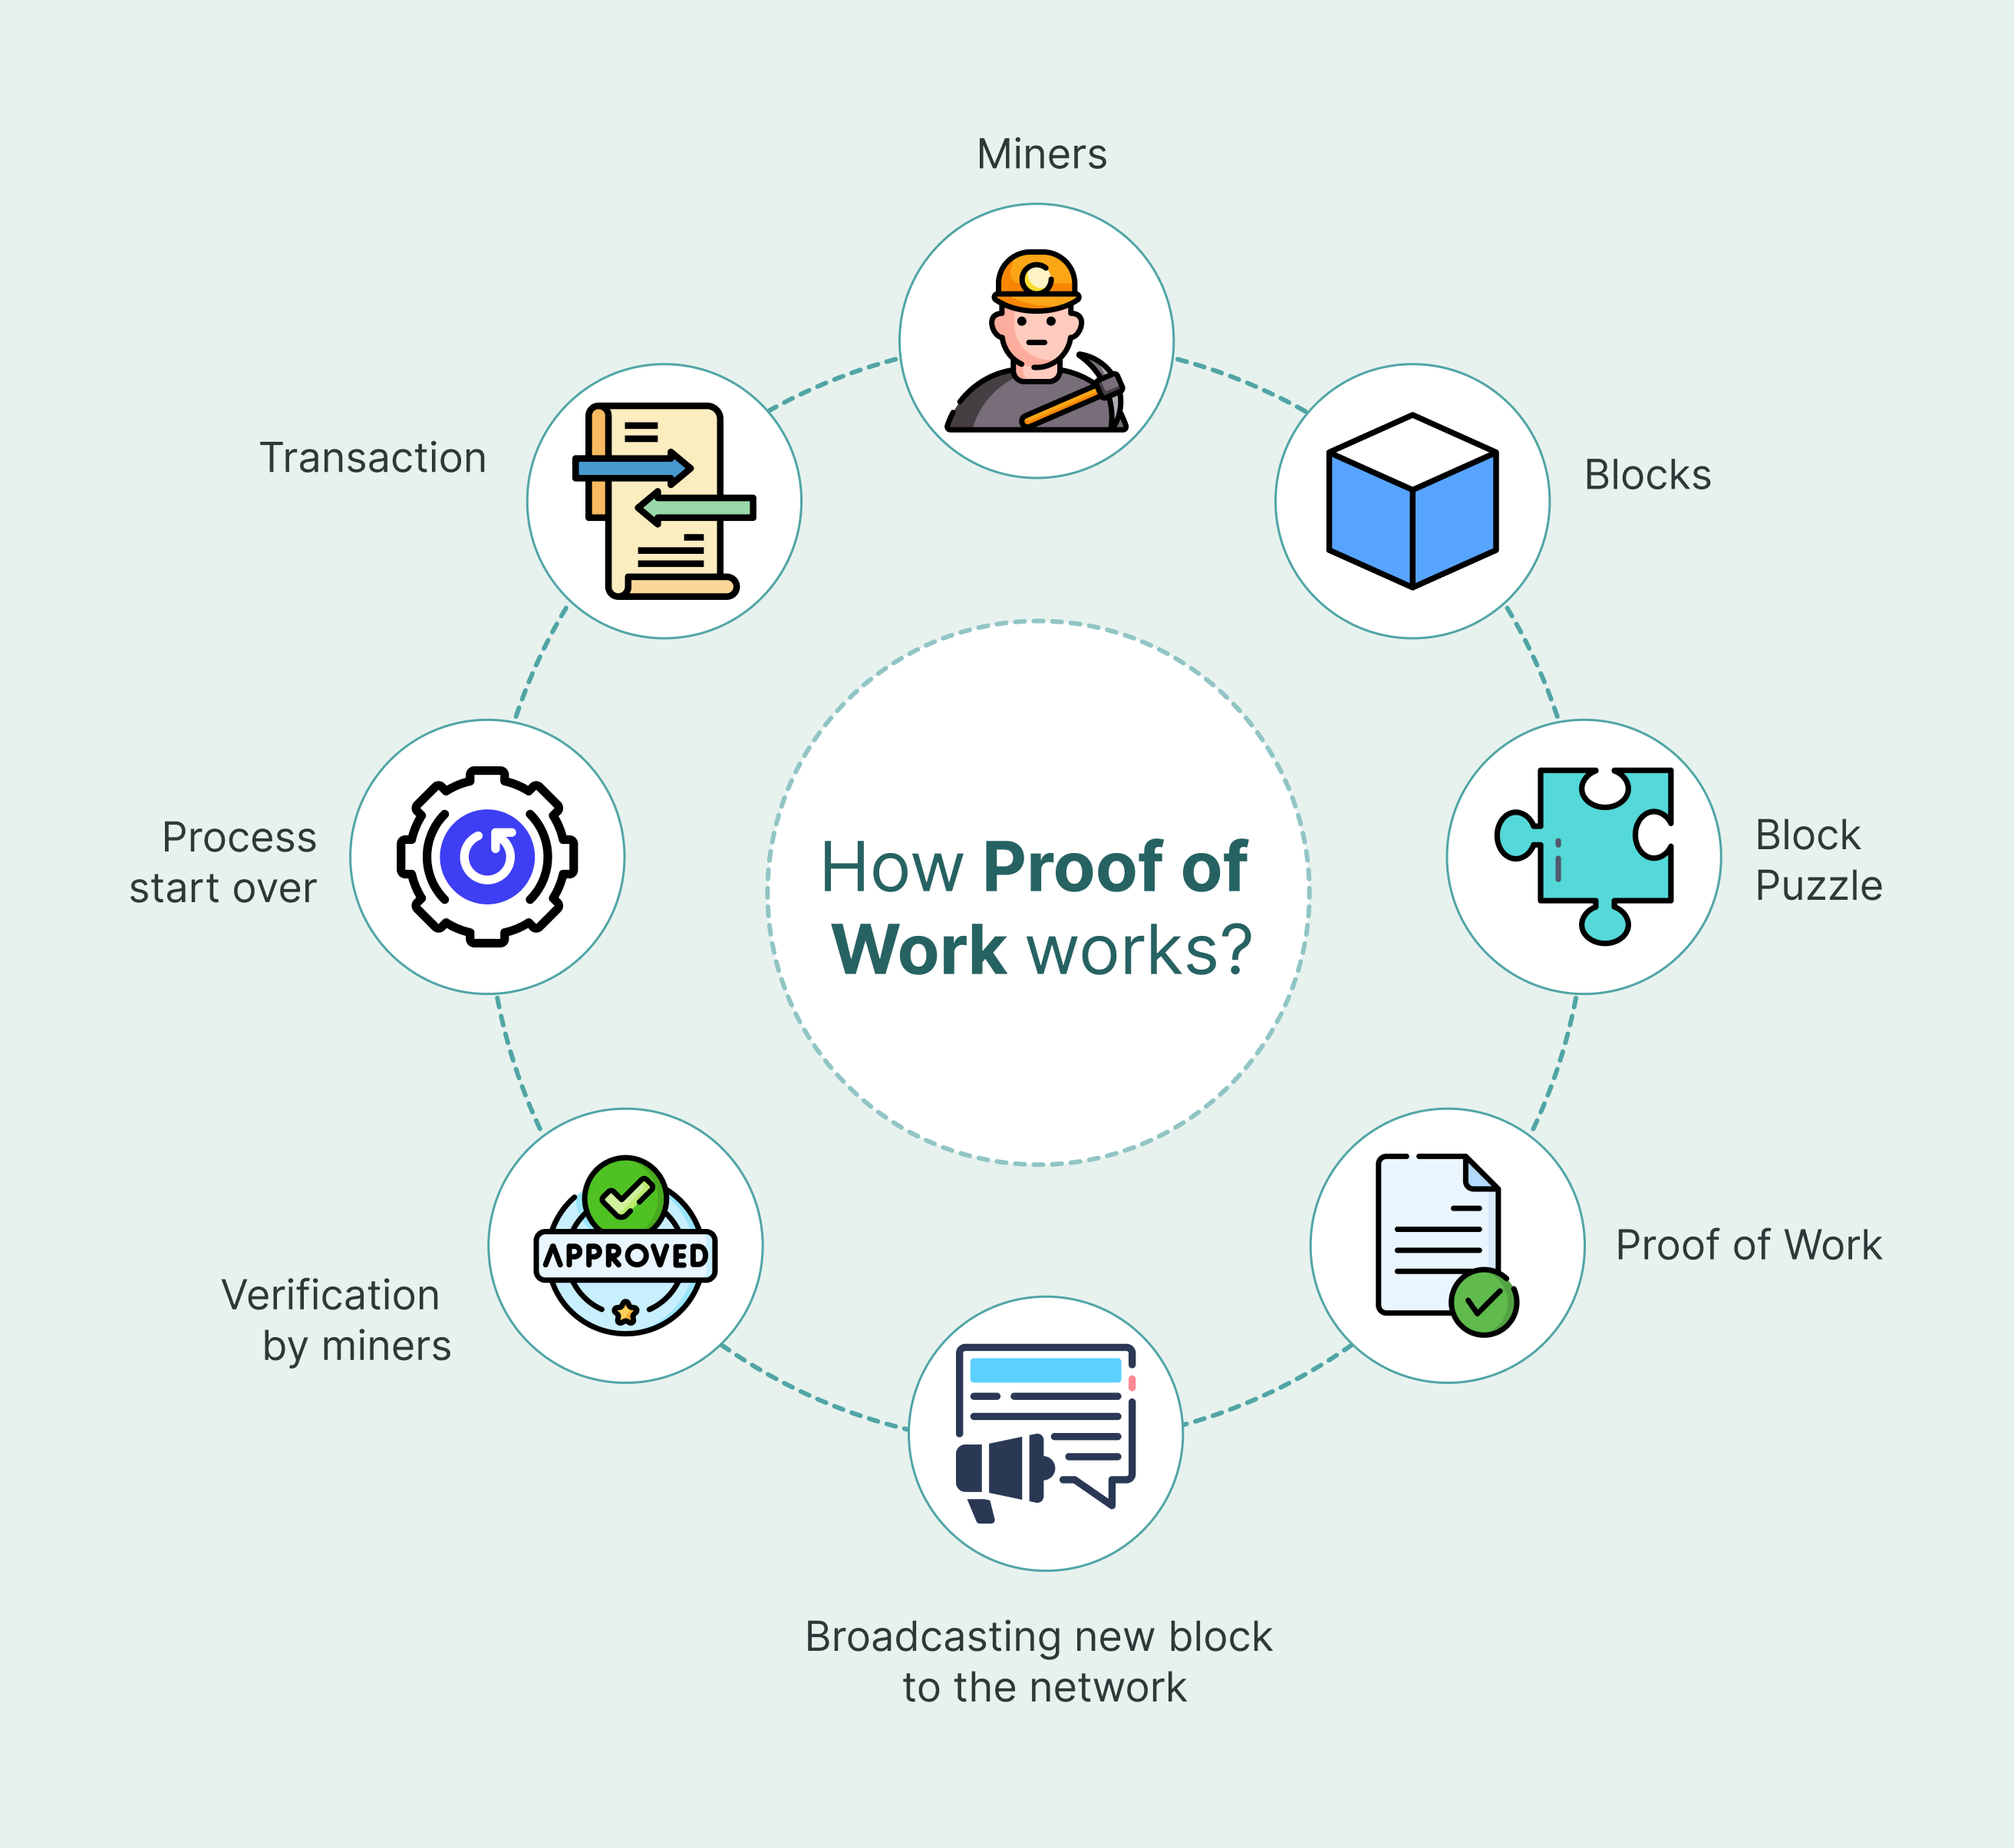
\includegraphics[width=\textwidth]{Images/ConsesnsusProofOfWork.png}
    \caption{Schemat działania Dowodu Pracy}
    \label{fig:ConsesnsusProofOfWork}
\end{figure}
\subsection{Dowód Stawki}
Dowód Stawki (angielski - Proof Of Stake) opiera się na założeniu, że im większą ktoś postawił/położył stawkę na to, że będzie mógł zostać wybrany weryfikatorem tym większe prawdopodobieństwo tego, że zostanie wybrany weryfikatorem. Szczegółowo mówiąc metoda Dowodu Stawki przebiega tak, że po zebraniu odpowiedniej liczby wiadomości tworzony jest blok, lecz aby mógł on zostać utworzony najpierw weryfikatorzy decydują czy wiadomości z bloku są autentyczne i nikt ich nieautoryzowanie nie zmodyfikował. Jeśli większość weryfikatorów postanowi, żeby zbiór wiadomości jest prawidłowy tworzony jest nowy blok. Weryfikatorzy, którzy głosowali uczciwie są nagradzani za swój głos poprzez podarowanie im określonej ilości kryptowaluty (angielski – stacking), a weryfikatorzy, którzy zagłosowali nieuczciwie karani są poprzez zabranie postawionej przez nich stawki (angielski – slashing). Wydawać by się mogło, że ta metoda promuje bogatych użytkowników i umożliwia im oszustwa, lecz w rzeczywistości osoby bogate (te który postawiły najwyższą stawkę) są najbardziej odstraszane od oszustwa, ponieważ w przypadku nieuczciwego zachowania podczas weryfikacji potencjalnego bloku są oni najbardziej karani (ponieważ postawili największą stawkę). Dodatkowo ta metoda konsensus zapewnia duży stopień decentralizacji (w przeciwieństwo do tego do czego w praktyce dochodzi w Dowodzie Pracy). W metodzie tej nie da się oszukać poprzez sytuację, że jedna osoba tworzy wiele kont (sytuacja określana też jako tworzenie multikont), ponieważ w metodzie konsensusu Dowodu Stawki nie chodzi o to ilu użytkowników jest w sieci, a ile postawili oni stawki.

\vspace{0.3\baselineskip}

Działanie Dowodu Stawki na grafice \ref{fig:ConsensusPOS}
\begin{figure}[H]
    \centering
    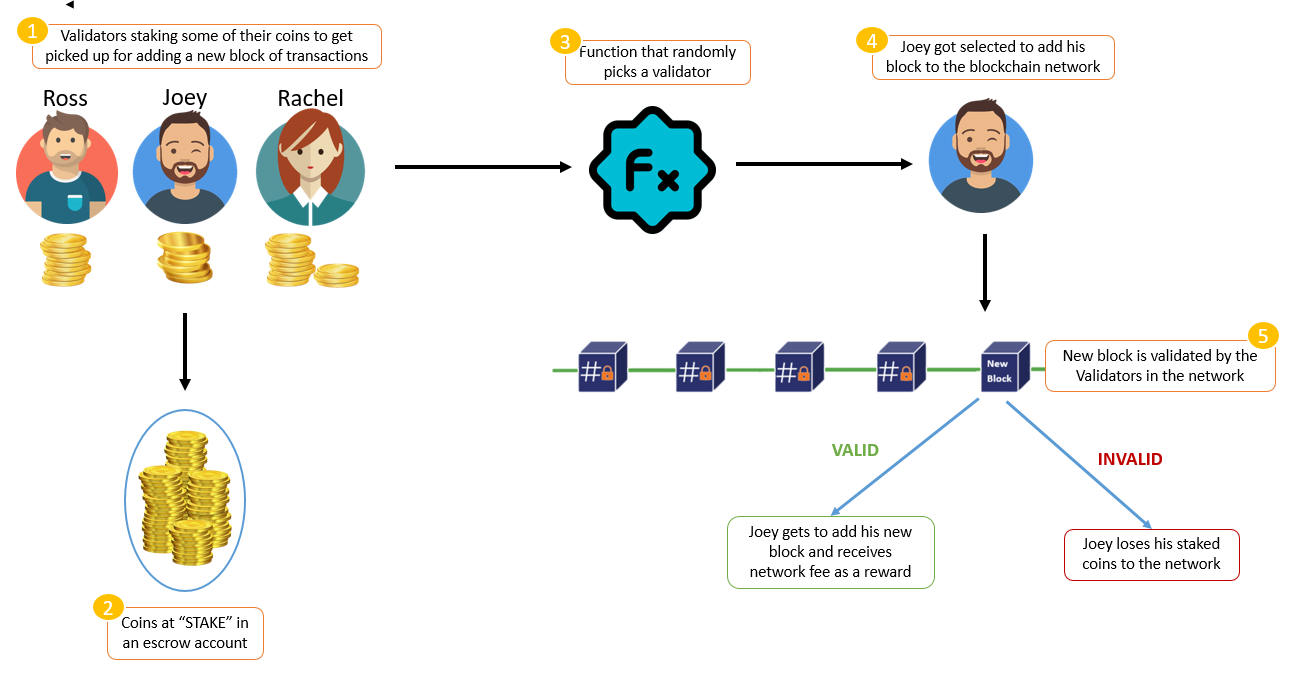
\includegraphics[width=\textwidth]{Images/ConsensusPOS.png}
    \caption{Schemat działania Dowodu Stawki}
    \label{fig:ConsensusPOS}
\end{figure}

\subsection{Delegowany Dowód Stawki}

Delegowany Dowód Stawki (angielski - Delegated Proof Of Stake) działa w podobny sposób jak Dowód Stawki, lecz z tym zastrzeżeniem, że wszyscy użytkownicy sieci zamiast mieć możliwość bycia wylosowanym głosują na jednego z dostępnych delegatów by on podczas weryfikacji głosował w ich imieniu. Nagrody za uczciwe głosowanie dostają delegaci, mogą podzielić się z nimi z użytkownikami, którzy na nich głosowali. Pomimo tego, że ta metoda konsensusu szybsza niż Dowód Stawki jej istotną wadą jest to, że w niej występuje o wiele większa centralizacji i zwykły użytkownik (o ile nie jest delegatem) nie ma bezpośredniej możliwości decydowania o tym czy uważa dany blok za prawidłowy czy też nie).

\vspace{0.3\baselineskip}

Działanie Delegowanego Dowodu Stawki na grafice \ref{fig:ConsensusDPOS}
\begin{figure}[H]
    \centering
    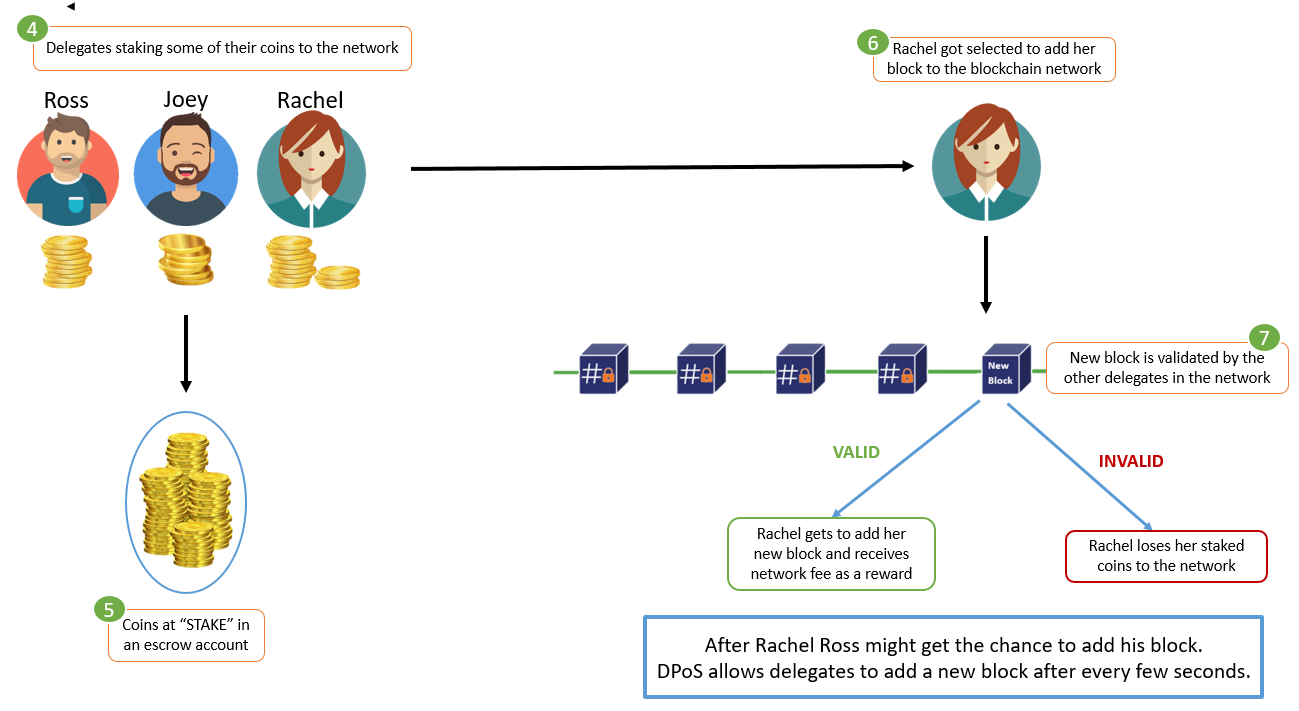
\includegraphics[width=\textwidth]{Images/ConsensusDPOS.png}
    \caption{Schemat działania Delegowanego Dowodu Stawki}
    \label{fig:ConsensusDPOS}
\end{figure}

\subsection{Dowód Pojemności}

W Dowodzie Pojemności (angielski - Proof Of Capacity) każdy z uczestników posiada pliki wykresów, w których są już wcześniej obliczone wartości matematyczne. Podczas tworzenia nowego bloku ogłaszana jest pewna wartość liczbowa i uczestnicy przeszukują swoje pliki wykresów, aby znaleźć wartość najbardziej do niej pasująca. Użytkownik, który będzie miał wartości najbliżej tej poszukiwanej zostanie nagrodzony kryptowalutą. Zaletą tej metody konsensusu jest fakt, że każdy może wziąć w niej udział, ale w rzeczywistości realne szanse mają osoby o ogromnej pojemności pamięciowej, co prowadzi do tworzenia się duży grup/związków tworzonych przez różne organizacje (na przykład firmy) co prowadzi do zwiększenia i dążenie do centralizacji.

\vspace{0.3\baselineskip}

Działanie Dowodu Pojemności na grafice \ref{fig:ConsensusPOC}
\begin{figure}[H]
    \centering
    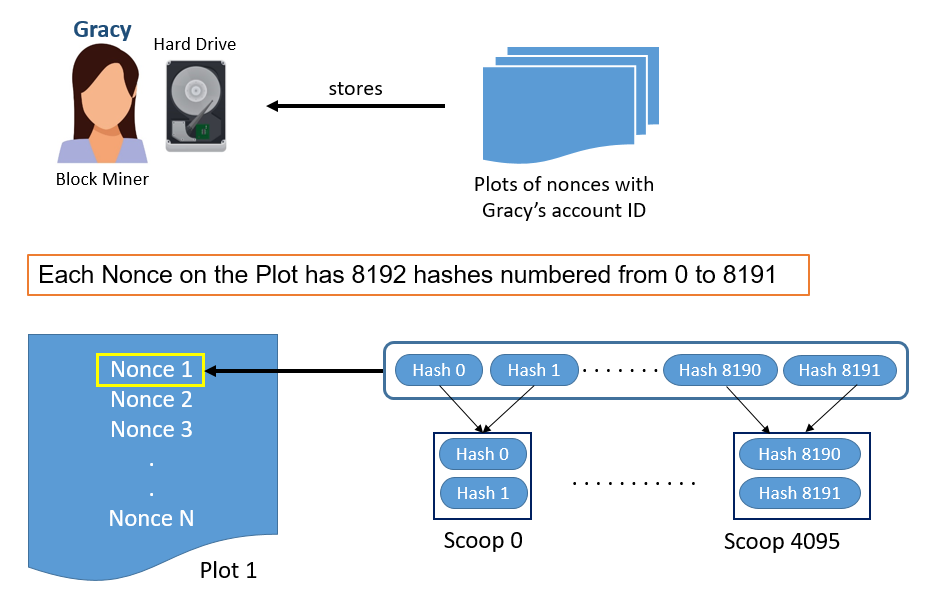
\includegraphics[width=\textwidth]{Images/ConsensusPOC.png}
    \caption{Schemat działania Dowodu Pojemności}
    \label{fig:ConsensusPOC}
\end{figure}

\subsection{Porównanie algorytmów osiągania konsensusu}
Spośród wszystkich dostępnych metod konsensusu wybrano tą która z pozoru wydaje się być nieuczciwie faworyzującą bogatszych uczestników. Dowód Stawki jest jedynym z wyżej wymienionych algorytmów, który nie ma w sobie istotnej wady jaką jest dążenie do centralizacji wywołane stosowaniem konkretnej metody konsensusu – centralizacji jednostek obliczeniowych (Dowód Pracy), centralizacji pojemności pamięciowej (Dowód Pojemności) czy centralizacji możliwość decydowania o poprawności danego bloku jedynie dla wybranej grupy osób (Delegowany Dowód Stawki). Dowód Stawki w przeciwieństwie do niektórych z innych algorytmów osiągania  konsensusu nie powoduje nadmiernego zużywania zasobów – prądu używanego do obliczeń w Dowodzie Pracy i przestrzeni dyskowej (w tym sprzętu elektronicznego) by zwiększyć ilość posiadanej pamięci w Dowodzie Pojemności. Wracając do zarzutu stawianego Dowodowi Stawki na początku akapitu co prawda najbogatsi (posiadający największą stawkę) mają największe szanse na zostanie weryfikatorem, ale w przypadku oszustwa są oni najmocniej karani, ponieważ tracą całą swoją postawioną stawkę (zjawisko to nazywa się slashing).

\subsection{Użycie algorytmów osiągania konsenusu w praktyce}
\begin{lstlisting}[caption={Wybieranie osoby mającej zostać weryfikatorem}]
def drawVerifier(self):
    personStakeList = []
    for peer in self.peers:
        personValue = {"addr": peer.addr, "port": peer.port,
        "stake": peer.stake}
        personStakeList.append(personValue)
    myValue = {"addr": ip(), "port": self.port, "stake": self.stake}
    personStakeList.append(myValue)
    personStakeList.sort(key=lambda x: x["port"])
    personSingleList = [{k: v for k, v in d.items() if k != "stake"} 
    for d in personStakeList]
    stakeSingleList = [x["stake"] for x in personStakeList]
    keyRaw = " ".join(str(x["port"]) for x in personStakeList)
    self.drawString = keyRaw
    numeric_seed = int.from_bytes(hashlib
    .sha256(keyRaw.encode('utf-8')).digest())
    random.seed(numeric_seed) #zmiana seeda dla losowania weryfikatora
    chosen_port = random.choices(personSingleList, 
    weights=stakeSingleList, k=1)[0]
    return chosen_port
\end{lstlisting}
\listings{Wybieranie osoby mającej zostać weryfikatorem}
Przy wybieraniu osoby, która będzie weryfikatorem korzysta się z funkcji, która ma go wyłonić kierując się zasadami z Dowodem Stawki. Problemem jaki nasuwa się przy implementowaniu funkcji jest to, jak sprawić, że każdy będzie miał wylosowanego tego samego weryfikatora, mimo tego, że uruchomienia programu są niezależne od siebie. Wywołanie u każdego z użytkowników zwykłej funkcji losującej wydaje się być nasuwającym się rozwiązaniem, lecz w rzeczywistości może doprowadzić to do sytuacji, gdzie różne osoby będę uznawały różnych członków sieci za weryfikatorów, co jest sytuacją, której chcemy uniknąć. Aby rozwiązać ten problem trzeba posłużyć się niezmiennikiem jakim jest założenie, że przy dowolnej komunikacji grupowej każdy z członków jest połączony z innymi użytkownikami w grupie (na tym polega rozmowa grupowa), ta sytuacja może być chwilowo zaburzona, ponieważ, łączenie się nie zawsze występuje w tym samym czasie, ale system domyślnie dąży do tego stanu.

\begin{lstlisting}[caption={Zamiana łańcucha znaków na wartość liczbową}]
numericSeed = int.from_bytes(hashlib.sha256(keyRaw
.encode('utf-8')).digest())
random.seed(numeric_seed)
\end{lstlisting}
\listings{Zamiana łańcucha znaków na wartość liczbową}

Dalej w kodzie z pozoru mało istotna funkcja skrótu, która zamienia łańcuch znaków na wartość liczbową. W rzeczywistości jest bardzo ważna, ponieważ jeśli jest ona niedeterministyczna (dla tego samego łańcucha znaków wylosuje ona różną wartość liczbową) to wyłanianie weryfikatora będzie mijać się z celem, bo wtedy nie wszyscy będą mieli tego samego weryfikatora. Skoro zostało wspomniane, dlaczego deterministyczna funkcja skrótu jest tak ważna, to warto wspomnieć, że domyślna funkcja skrótu w Pythonie – hash() – nie jest funkcją deterministyczną, ponieważ wprowadzono do niej mechanizm losowości skrótu (angielski - hash randomization) który dodaje do funkcji skrótu losową ,,sól”. Z tego powodu w systemie zastosowano metodę hashlib.sha256(), która jest deterministyczna. Następnie tak utworzoną liczbą ustawiamy ziarno generatora liczb pseudolosowych tak, aby generator dla tych samych danych wejściowych dał nam takie same wyniki.

\begin{lstlisting}[caption={Losowanie weryfikatora}]
chosen_port = random.choices(personSingleList, 
weights=stakeSingleList, k=1)[0]
return chosen_port
\end{lstlisting}
\listings{Losowanie weryfikatora}

Następnie odbywa się losowanie weryfikatora, jako zgodne z metodą uzyskania konsensusu Dowodu Stawki jest wylosowanie jednego z uczestników, ale nie za pomocą zwykłej metody random.choice w Pythonie, która losowałaby elementy z listy z równym prawdopodobieństwem, ale z metodą random.choices, której argumentem (poza listą członków sieci), jest lista wartości postawionych przez nich jako stawki i jest ona stosowana jako lista wag, to znaczy im ktoś większą postawił stawkę, tym większa jest jego szansa na zostanie wylosowanym, co jest zgodne z założeniami Dowodu Stawki.

\section{Metody zabezpieczania bloku}

Gdy zestaw wiadomości został zweryfikowany jako prawidłowy i tworzony jest z nich blok, pojawia się wątpliwość jak zabezpieczyć blok przed nieautoryzowanymi zachowaniami  (zmianami treści wiadomości), tak aby każdy członek sieci mógł w łatwy sposób sprawdzić czy faktycznie, nikt nie zmodyfikował wiadomości (na przykład w celu oszustwa, które ma mu przynieść korzyść).

\subsection{Zabezpieczanie bloku w Dowodzie Pracy}

W metodzie konsensusu Dowód Pracy poprawność bloku sprawdza się poprzez porównywanie funkcji skrótu odpowiednio ze sobą połączonych bloków. Wadą tego rodzaju rozwiązania jest fakt, że do samego sprawdzenia podpisu potrzebne są ogromne moce obliczeniowe, co jest mocno nie korzystne i dodatkowo jednostka lub zespół jednostek posiadający odpowiednio dużą moc obliczeniową może zamienić treści wiadomości w poprzednich blokach w łańcuchu tak, aby wartość funkcji skrótu się zgadzała z nowszymi wiadomościami i nie wzbudzała podejrzeń.

\vspace{0.3\baselineskip}

Łączenie bloków w Dowodzie Pracy za pomocą funkcji skrótów na grafice \ref{fig:ProofOfWorkHash}
\begin{figure}[H]
    \centering
    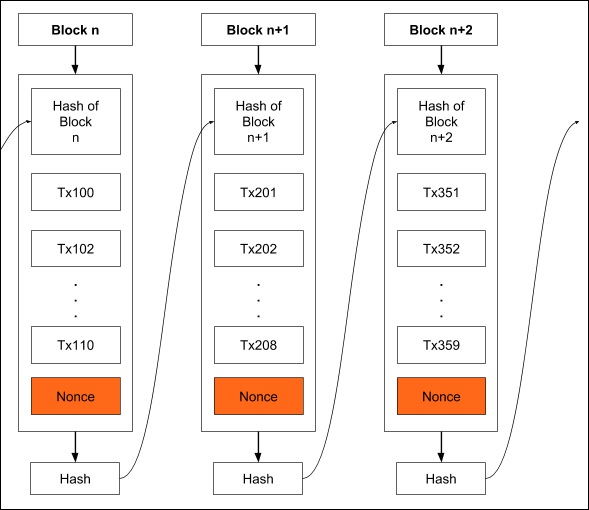
\includegraphics[width=\textwidth]{Images/ProofOfWorkHash.jpg}
    \caption{Działanie funkcji skrótu w Dowodzie Pracy}
    \label{fig:ProofOfWorkHash}
\end{figure}

Zamiast stosować skomplikowany połączonych ze sobą funkcji skrótu w implementacji systemu postanowiono skorzystać z innej metody, również stosowanej w innych systemach kryptograficznych. Jest to podpis cyfrowy.

\subsection{Zabezpieczanie bloku poprzez podpis cyfrowy}

Podpis cyfrowy opiera się na kryptografii asymetrycznej, gdzie każdy z użytkowników ma dwa klucze – klucz publiczny i klucz prywatny. W podpisie cyfrowym najpierw wykonuje się funkcję skrótu (w implementacji stosuje się SHA-256) na danych znajdujących się w bloku. Potem tą wartość szyfruje się kluczem prywatnym. Podpis cyfrowy (w przeciwieństwie do szyfrowania) jest wykonywany kluczem prywatnym, ponieważ jeśli weryfikator po otrzymaniu wartości funkcji skrótu próbował podpisać ją kluczem publicznym to żaden z użytkowników nie miałby możliwości zweryfikowania takiego podpisu, ponieważ do to tego potrzebny jest drugi klucz, czyli klucz prywatny, ale założeniem kryptografii asymetrycznej jest to, że klucz prywatny jest niedostępny dla innych. 

Zilustrowanie podpisu cyfrowego na grafice \ref{fig:DSJP}:
\begin{figure}[H]
    \centering
    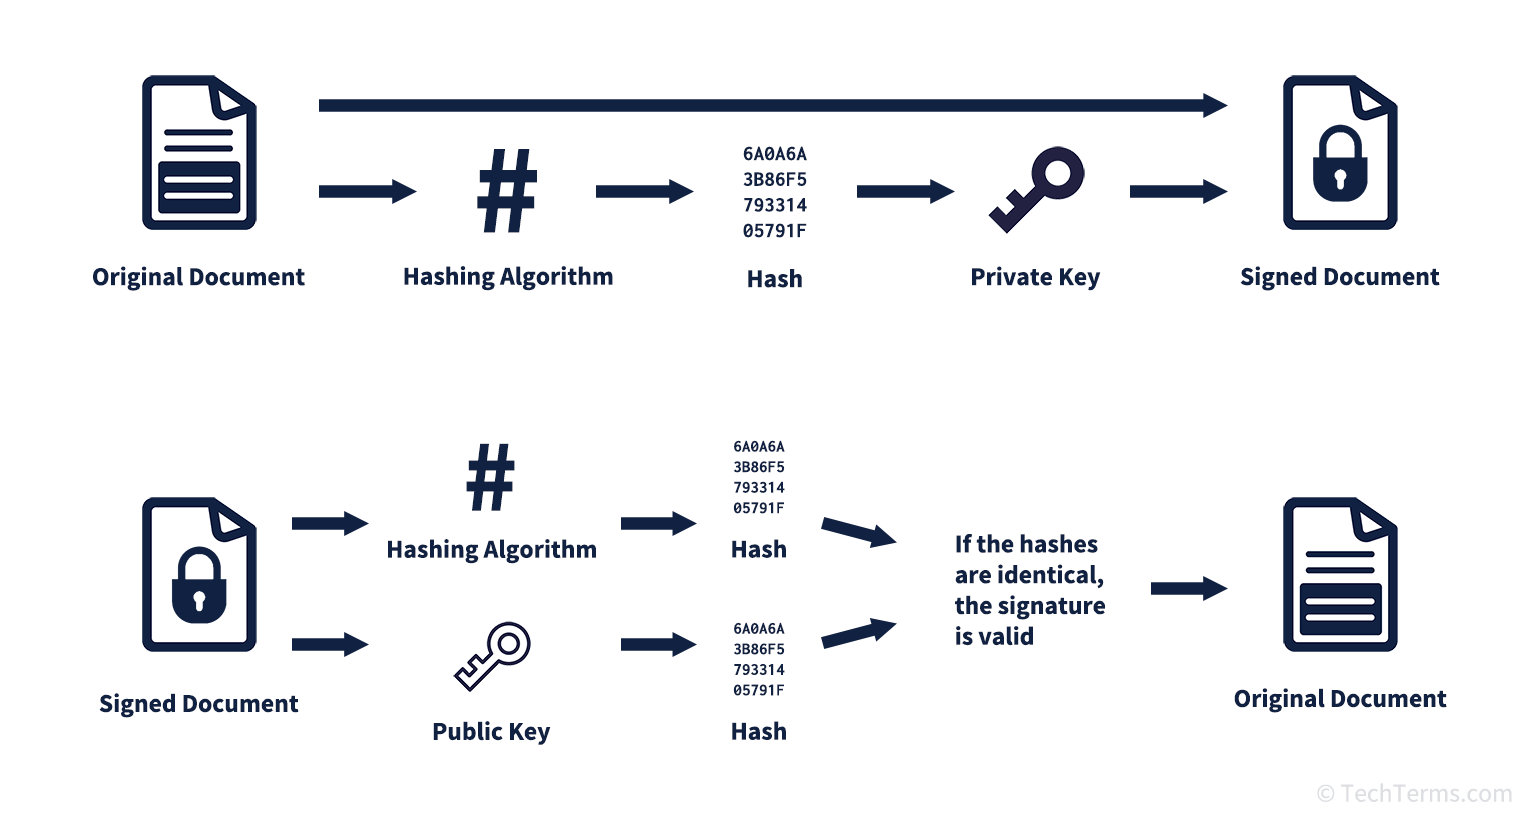
\includegraphics[width=\textwidth]{Images/DSJPG.jpg}
    \caption{Działanie podpisu cyfrowego}
    \label{fig:DSJP}
\end{figure}

Aby zweryfikować podpis cyfrowy należy wygenerować hash z danych znajdujących się w bloku. Jeśli ta wartość jest tożsama z wartością podpisu cyfrowego odszyfrowanego kluczem publicznym twórcy podpisu to znaczy, że podpis jest autentyczny.

\subsection{Zabezpieczanie bloku w praktyce}

\begin{lstlisting}[caption={Wysyłanie podpisu elektronicznego}]
def sendDigitalSignature(self, ListOfJSON, me):
    jsonMessages = self.get_messages_block(ip())
    drawnVerifier = self.drawVerifier()
    if drawnVerifier == self.port:
        me.remove_single_message_JSON(ip())
        for count, jsonSingleMessage in enumerate(jsonMessages):
            if jsonMessages[count] == ListOfJSON[0]:
                length = len(ListOfJSON)
                identicalResult = jsonMessages[count:count+length]
                                == ListOfJSON
                if identicalResult:
\end{lstlisting}
\listings{Wysyłanie podpisu elektronicznego}
Jeżeli dany użytkownik został wylosowany jako weryfikator, a następnie jeśli otrzymane wiadomości (od osoby wysyłającej ostatnią wiadomość w bloku) zgadzają się z wiadomościami, które posiada weryfikator to potwierdza je on za pomocą wystawienia podpisu cyfrowego.

\begin{lstlisting}[caption={Tworzenie podpisu elektronicznego}]
def createSignature(self, dataStrng):
    data = dataStrng.encode('utf-8')
    signature = self.private_key.sign(
        data,
        padding.PKCS1v15(),
        hashes.SHA256()
    )
    return signature
\end{lstlisting}
\listings{Tworzenie podpisu elektronicznego}
Następnie tworzony jest podpis cyfrowy na podstawie przekazanych wiadomości w formie łańcucha znaków. Szczegółowo, że łańcuch znaków przekształcany jest do postaci binarnej, potem te dane binarne są podpisywane przy wykorzystaniu klucza prywatnego. Poza samymi danymi innymi argumentami w schemacie podpisu cyfrowego jest wypełnienie (angielski – padding) – tu używane jest schemat PKCS1v15. Innym argumentem do funkcji podpisu cyfrowego jest określona funkcja skrótu, ponieważ podpisywanie całego ciągu znaków binarnych byłoby zbyt czasochłonne, w tym przypadku zastosowano algorytm SHA256. Podczas implementacji może pojawić się wątpliwość czy każdy z użytkowników będzie mógł dla tych samych danych otrzymać taki sam podpis cyfrowy i czy przy weryfikacji podpisu cyfrowego dla tych samych danych otrzyma ten sam wynik. Jest to kluczowe dla działania programu, jeśli to nie zostałoby to zapewnione weryfikacji podpisu cyfrowego byłaby nie możliwa. Pożądana przez nas cecha algorytmu, czyli fakt, że dla tych samych danych algorytm zawsze zwróci ten sam wynik to deterministyczność. Jak sprawdzić czy nasz podpis cyfrowy jest deterministyczny – trzeba dowiedzieć się czy funkcja go tworząca zwraca deterministyczny wynik, a faktem jest informacja, że w tej funkcji jest to uzależnione od tego jakie wypełnienie jest stosowane oraz jaki algorytm generowania funkcji skrótu jest stosowany. Co do metody wypełnienia PKCS1v15 – jest ona deterministyczna (nie stosuje ona elementów losowanych w przeciwieństwie do wielu innych metod wypełnienia), funkcja skrótu SHA256 (w przeciwieństwie do niektórych innych funkcji skrótu) jest deterministyczna. Ukazując, to że metoda wypełnienia jak i funkcja skrótu są deterministyczne, ukazane jest, że funkcja generująca podpis cyfrowy, która od nich bezpośrednio zależy również jest deterministyczna, więc udowodniono, że podpis cyfrowy jest deterministyczny (taki sam dla identycznych danych wejściowych).

\section{Algorytmy kodowania transportowego}
\subsection{Opis algorytmów kodowania transportowego}
Podczas przesyłania danych przez sieć może pojawić się problem, że niektóre dane (na przykład podpis cyfrowy czy klucz publiczny) są w postaci ciągu bajtów. Ich przesyłanie przez sieć w formie binarnej jest dość problematyczne, więc dobrym rozwiązaniem problemu jest ich przekonwertowanie na format danych, który można w łatwiejszy sposób przesłać jak na przykład łańcuch znaków. Można wykonywać to ręcznie, ale lepszym rozwiązaniem jest skorzystanie z gotowego algorytmu kodowania transportowego. Istnieje wiele algorytmów kodowania transportowego, takie jak Base16, Base32, Base36, Base62 czy Base64 czy Base85. W implementacji projektu został wybrany jeden z najbardziej znanych i efektywnych algorytmów kodowania transportowego, czyli Base64. Jego działanie polega na tym, że dzieli on ciąg bajtów na trzy-bajtowe grupy, które są potem dzielone na cztery sześciobitowe grupy, a każda z tych sześciobitowych grup jest zamieniana na jedną liczbę. Liczba ta jest uzyskiwana mnożąc bity od najmłodszego do najstarszego przez kolejną potęgę liczby dwa według wzoru \ref{eq:Base64Formula}
\begin{equation}
    Liczba = \sum_{i=1}^6 bit_i * 2^{i-1}
    \label{eq:Base64Formula}
\end{equation}
\equations{Liczba w kodowaniu Base64}
Podział ciągu bajtów na trzybajtowe grupy, na następnie na cztery sześciobitowe grupy został zwizualizowany, na grafice \ref{fig:Base64Schema}
\begin{figure}[H]
    \centering
    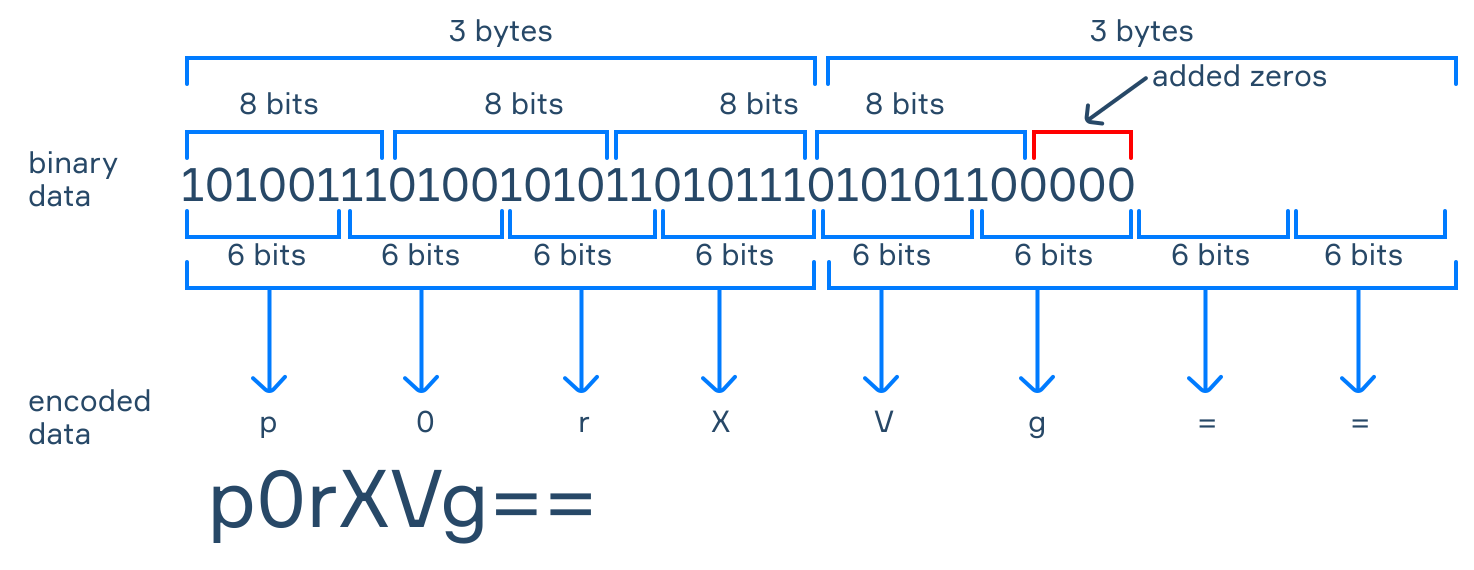
\includegraphics[width=\textwidth]{Images/Base64Schema.png}
    \caption{Schemat Base64}
	\label{fig:Base64Schema}
\end{figure}
Potem liczba ta konwertowana jest na jeden z sześćdziesięciu czterech znaków ASCII (jest to cyfra od 0 do 9, albo wielka litera od A do Z, albo mała litera od a do z, albo znak plusa lub równości). Odbywa się to zgodnie ze schematem pokazanym na grafice \ref{fig:Base64Coding}
\begin{figure}[H]
    \centering
    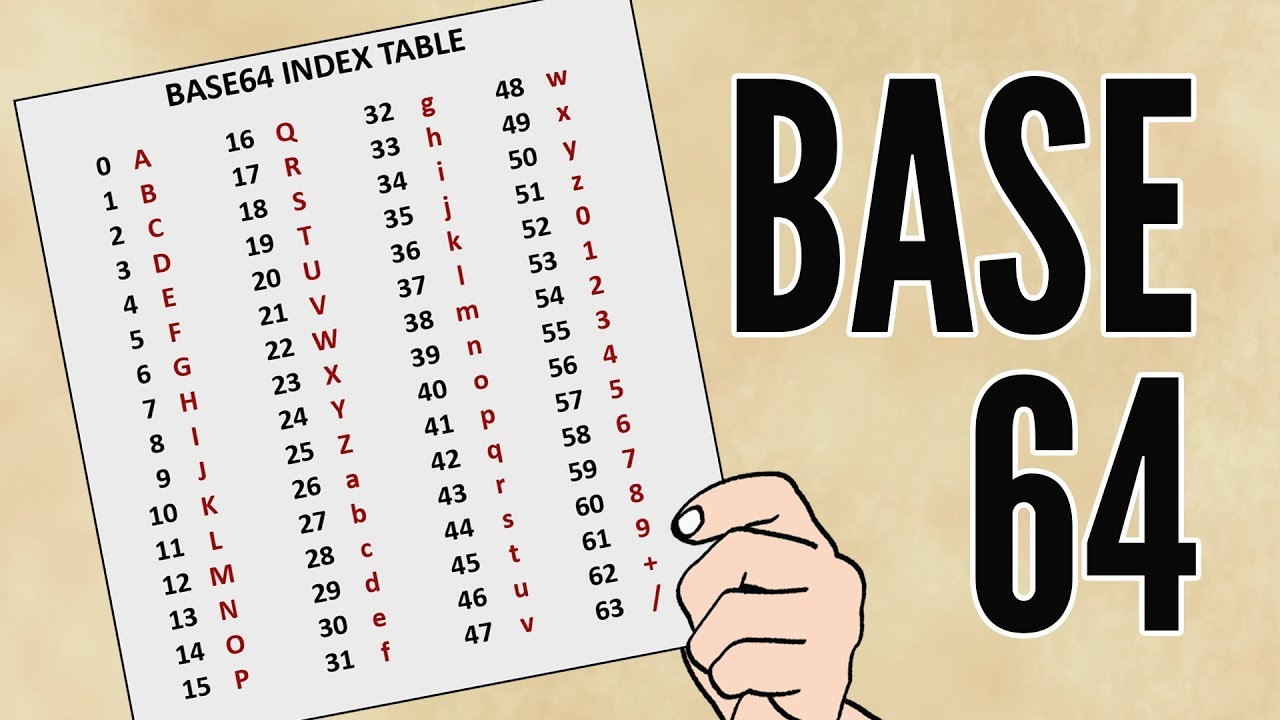
\includegraphics[width=\textwidth]{Images/Base64Coding.jpg}
    \caption{Kodowanie w Base64}
	\label{fig:Base64Coding}
\end{figure}
Na ciągu znaków w formacie Base64 można również wykonać operację odwrotną, czyli zdekodować go do postaci binarnej.

\vspace{0.3\baselineskip}

Jeśli długość ciągu bajtów nie jest liczbą podzielną przez trzy stosuje się dopełnienie, która zamiast wcześniej opisanych sześdziesięciu czterech znaków dodaje znaki równości tak, żeby liczba znaków po konwersji była liczbą podzielną przez cztery.
\chapter{Interfejs graficzny użytkownika}
\label{chap:InterfejsGraficznyUżytkownika}
Aplikacja posiada rozbudowany graficzny interfejs użytkownika, który w sposób responsywny dostosowuje się do urządzeń desktopowych oraz mobilnych. Interfejs dostępny jest w dwóch trybach wizualnych: jasnym i ciemnym, oferując różnorodne efekty kolorystyczne oraz animacje. Dodatkowo aplikacja renderuje dynamicznie pojedynczy obiekt trójwymiarowy wraz z jego animacją, co wzbogaca wizualny aspekt interfejsu.

%---
\section{Projektowanie interfejsu graficznego}
\label{sec:ProjektowanieInterfejsuGraficznego}

\emph{Projektowanie interfejsu graficznego \ang{UI Design}}, to proces tworzenia wizualnego środowiska użytkownika przed jego implementacją programistyczną. W ramach naszego projektu inżynierskiego wykorzystałem profesjonalne narzędzie Figma \cite{Figma} do zaprojektowania interfejsu graficznego użytkownika, co pozwoliło usprawnić i ujednolicić dalsze prace związane z implementacją tego interfejsu w kodzie. Projekt graficzny stworzony w Figmie pełnił funkcję przewodnika, przy programowaniu interfejsu.

%---

\subsection{System Projektowania}
\label{sec:SystemProjektowania}

\emph{System projektowania \ang{Design system}}, to zestaw standaryzowanych danych i zasobów projektowych, które wspólnie definiują wygląd interfejsu graficznego i usprawniają proces projektowania. Celem Design systemu jest zapewnienie spójności wizualnej oraz ułatwienie współpracy między członkami zespołu. 
W ramach projektowania interfejsu graficznego, zacząłem od stworzenia prostego systemu projektowania, który ujednolicił paletę barw, definiując zestawy kolorów o różnych odcieniach jasności, rozmiary czcionek oraz odstępy między elementami. Te wartości stałe były konsekwentnie wykorzystywane zarówno w procesie projektowania, jak i w implementacji interfejsu graficznego, zapewniając spójność wizualną i funkcjonalną. 

%---

\subsection{Proces projektowania}
\label{sec:ProcesProjektowania}
Po zdefiniowaniu Systemu Projektowania rozpocząłem projektowanie stron aplikacji w dwóch rozdzielczościach: 1440x1024 dla urządzeń desktopowych oraz 375x667 dla urządzeń mobilnych. Dla każdej z tych rozdzielczości przygotowałem dwie wersje stron, różniące się układem elementów. Wszystkie projekty początkowo powstawały w kolorystyce \ang{Dark Mode}, a następnie były tworzone ponownie w jasnej wersji \ang{Light Mode}.

%---

\section{Implementacja Interfejsu Graficznego}
\label{sec:ImplementacjaInterfejsuGraficznego}
Język Python posiada wiele bibliotek do tworzenia interfejsów graficznych, nasz zespół zdecydował się na użycie frameworka QT w wersji 6 (Pyside6). Dzięki temu, że framework stanowi pakiet w języku Python nasz zespół mógł używać różnych IDE \ang{Integrated Development Environment}.
Framework ten posiada wiele narzędzi i komponentów umożliwiających tworzenie nie tylko interfejsów graficznych, od własnych struktur danych po moduły do pracy z bazami danych, jednakże w naszym projekcie głównie korzystaliśmy z języka Qt do Modelowania (QML) \ang{Qt Modeling Language} - deklaratywnego języka do tworzenia interfejsów w Frameworku QT. QML oraz QT jest wieloplatformowy, działa na urządzeniach desktopowych (Windows, Linux, MacOS) oraz urządzeniach mobilnych i wiele innych.
Dzięki QML możliwe było logiczne rozdzielenie backendu i frontendu, co pozwoliło na zapisanie definicji interfejsu graficznego w odrębnych plikach z rozszerzeniem .qml, ułatwiając tym samym zarządzanie kodem i jego strukturą.

\subsection{Uzasadnienie wyboru Frameworka QT}
\label{sec:UzasadnienieWyboruFrameworkaQT}
Przy wyborze technologii do tworzenia interfejsów graficznych w Pythonie mieliśmy do wyboru wiele innych bibliotek, na przykład Tkinter. 
Jednakże w porównaniu do Tkintera, interfejsy w tej bibliotece są przestarzałe wizualnie i mniej elastyczne. Biblioteka ta oferuje małe wsparcie dla chociażby efektów wizualnych, animacji czy responsywnego designu.

Framework QT oraz zawarty w nim QML mają wiele zalet, które nas przekonały do skorzystania z tej technologii:
\begin{enumerate}
    \item Qt jest wieloplatformowy, można tworzyć aplikacje na Windowsa, Linuxa, MacOSa i urządzenia mobilne
    \item Łatwo łączyć logikę backendu z frontendem
    \item QML umożliwia dodawanie animacji, renderowanie obiektów trójwymiarowych i tworzenie responsywnego interfejsu
    \item QT posiada ogromną dokumentację i ma szeroką społeczność użytkowników
    \item Oddzielenie frontendu (QML) od backendu (Python) sprzyja lepszej organizacji kodu
\end{enumerate}

\subsection{Podstawy QT Modeling Language} 
\label{sec:PodstawyQtModelingLanguage}
\emph{Qt Modeling Language} to język deklaratywny podobny do CSS i HTML, wchodzący w skład modułu QtQuick frameworka Qt. Aby zacząć używać QML'a, należy stworzyć plik .qml w którym możemy zawrzeć:

\begin{lstlisting}[language=QML, caption={Przykładowy kod QML}]
import QtQuick 2.0

Rectangle {
    id: kwadrat
    width: 100
    height: 100
    color: "red"
}
\end{lstlisting}
który tworzy kwadrat 100x100 w kolorze czerwonym, struktura kodu w QML jest hierarchiczna oznacza to, że wewnątrz kodu Rectangle moglibyśmy dodać kolejny obiekt, który byłby tworzony względem rodzica - Rectangle.

Dodatkowo QML umożliwia pisanie w języku Javascript w odpowiednich polach,
na przykład do kodu w kwadracie można dodać:

\begin{lstlisting}[language=QML, caption={Przykładowy Javascript}]
Component.onCompleted: {
    console.log(kwadrat.width);
}
\end{lstlisting}
który wypisze w konsoli szerokość kwadratu.


\subsection{Zaimplementowane istotne mechanizmy}
\label{sec:ZaimplementowaneIstotneMechanizmy}

\subsubsection{Struktura Interfejsu}
\label{sec:Struktura Interfejsu}
W naszym projekcie każdy osobny plik .qml stanowi osobną stronę interfejsu lub
definicję niestandardowego komponentu. Niestandardowe komponenty są zawarte
w osobnych folderach: \begin{lstlisting}
"app_style", "gui_components", "small_gui_components"
\end{lstlisting}

Omówię najpierw aspekt niestandardowych komponentów. W QMLu można tworzyć własne klasy komponentów.

\begin{lstlisting}[language=QML, caption={Przykładowa klasa w MyRectangle.qml}]
MyRectangle {
    id: rectangle
    color: "blue"
    width: 100
    height: 100
}
\end{lstlisting}
Zaimportowanie tego w innym pliku (Page1.qml) umożliwi stworzenie
wielu instancji klasy MyRectangle:

\begin{lstlisting}[language=QML, caption={Przykładowe użycie klasy MyRectangle}]
MyRectangle {} //niebieski kwadrat 100x100
MyRectangle {color: "red"} //czerwony kwadrat 100x100
\end{lstlisting}
Pozwala to na uniknięcie redundancji w kodzie, gdy trzeba tworzyć
wiele obiektów, różniących się, tylko niektórymi atrybutami.

W naszym projekcie jest to wykorzystywane przy tworzeniu list, na przykład
użytkowników albo własnych przycisków, których w interfejsie jest pełno i dzięki definiowaniu ich w jednej klasie, wyglądają podobnie i upraszczają kod.

Reszta plików \texttt{.qml} stanowi osobne strony interfejsu. 
Tworząc komponent StackView oraz używając:
\begin{lstlisting}[language=QML, caption={Ładowanie nowej strony}]
stackView.push("nazwa_pliku.qml");
\end{lstlisting}
można w bardzo prosty sposób załadować nową stronę.
Taki podział (strona - plik) sprawia, że struktura interfejsu jest bardziej
uporządkowana oraz logiczna i upraszcza pracę z kodem.

\subsubsection{Implementacja Systemu Projektowania}
\label{sec:ImplementacjaSystemuProjektowania}
System Projektowania z części Projektowania Interfejsu Graficznego zakłada użycie stałej palety kolorów, odstępów oraz wielkości czcionek.

Nasz projekt implementuje to w folderze \texttt{app\_style} w trzech plikach QML:

\begin{enumerate}
    \item ColorPalette.qml - Definiujący zestaw stałych kolorów
    \item FontStyle.qml - Definiujący czcionkę oraz różne rozmiary
    \item SpacingObjects.qml - Definiujący wartości odstępów między elementami w interfejsie
\end{enumerate}

Każdy z nich zawiera analogiczną logikę, więc omówię na przykładzie klasy \texttt{ColorPalette}:

W kodzie QML definiujemy stałe zmienne przy użyciu \texttt{property}

\begin{lstlisting}[language=QML, caption={ColorPalette.qml}]
import QtQuick 2.15

QtObject {
    readonly property color primary50: "#EBFFE5"
    readonly property color primary100: "#D7FFCC"
    readonly property color primary200: "#AFFF99"
    readonly property color primary300: "#87FF66"
    readonly property color primary400: "#5FFF33"
    readonly property color primary500: "#37FF00"
    readonly property color primary600: "#2CCC00"
    readonly property color primary700: "#219900"
    readonly property color primary800: "#166600"
    readonly property color primary900: "#0B3300"

    readonly property color secondary50: "#FEE5FF"
    readonly property color secondary100: "#FDCCFF"
    ...
    ...
\end{lstlisting}

Następnie w bardzo prosty sposób możemy używać tych stałych wartości w każdym miejscu w kodzie:
\begin{lstlisting}[language=QML, caption={Przykładowe użycie palety kolorów}]
import "../app_style"

//User (Peer) List Class Blueprint
Rectangle {
ColorPalette { id: colorPalette }
FontStyle { id: fontStyle }
SpacingObjects { id: spacingObjects }

    property string list_color: settings.light_mode ? colorPalette.background50 : colorPalette.background800
    ...
    ...
\end{lstlisting}  

\subsubsection{Komunikacja z Backendem}
\label{sec:KomunikacjaZBackendem}
Komunikacja z backendem w Frameworku QT odbywa się za pomocą sygnałów i slotów. Ten sam mechanizm istnieje również, gdy używamy QT wraz z językiem C++, jednakże syntax jest inny. 

Sygnał to obiekt, który jak nazwa wskazuje ma za zadanie wysłanie sygnału,
dokonuje się tego przy pomocy metody .emit().

Slot to specjalna funkcja, którą należy połączyć z wybranym, uprzednio stworzonym sygnałem.

Po wysłaniu sygnału zostaje wywołany ten podłączony Slot. Dodatkowo można przesyłać w metodzie .emit() argumenty do Slota.

Jeżeli chcemy osiągnać komunikację między backendem (plikami .py) oraz frontendem (.qml) to logicznie:

\begin{enumerate}
    \item Definiujemy sygnał w klasie w Pythonie, który potem należy podłączyć do zdefiniowanej w QML-u za pomocą JavaScript funkcji (slota) i następnie wywołać \texttt{.emit()} z poziomu Pythona dla tego sygnału. To umożliwi wywołanie funkcji zawartej w QML za pomocą kodu w Pythonie.
    \item Możemy też pójść w drugą stronę – jeśli chcemy wywołać coś z backendu przy użyciu kodu QML, wtedy należy stworzyć slot w klasie w Pythonie, gdzie kod QML staje się sygnałem.
\end{enumerate}

Istotnym aspektem jest to, że samo przekazanie wartości do frontendu jest operacją prostą, można tego dokonać jednorazowo przy inicjalnym ładowaniu interfejsu, o czym za chwilę, jednakże mechanizm sygnałów i slotów umożliwia dynamiczne przekazywanie informacji między frontendem i backendem.

Na przykład jeśli dodamy kogoś do znajomych, to w backendzie w funkcji która odpowiada za dodanie użytkownika do znajomych możemy wywołać .emit() i dynamicznie obsłużyć tą zmianę we Frontendzie.

Teraz pokazując kod z naszego projektu omówię na przykładzie jak wykorzystaliśmy ten mechanizm:

Przykładowo jeśli dynamicznie obsłużyć zmianę znajomych w naszym programie, to atrybut self.peers w klasie User() w Backendzie zawiera tablicę innych obiektów typu User, które chcemy przekazać do Frontendu i wypisać na ekranie.

Tworzymy sygnał w klasie User:
\begin{lstlisting}[language=Python, caption={Sygnał User}]
class User(QObject):
    peersChanged = Signal()
\end{lstlisting}    

Definiujemy tablicę peers jako Property:
\begin{lstlisting}[language=Python, caption={Peers Property}]
@Property("QVariantList", notify=peersChanged)
    def peers(self):
        return self._peers
\end{lstlisting}

W main.py przed inicjalnym załadowaniem interfejsu możemy przekazać
uprzednio stworzony pojedyńczy obiekt User, gdzie u nas jest to obecny użytkownik programu. Teraz w QML możemy używać metod i atrybutów tej klasy dla tego obiektu.

\begin{lstlisting}[language=Python, caption={Przekazanie inicjalnego obiektu}]
engine.rootContext().setContextProperty("user", user)
\end{lstlisting}

Teraz w klasie FriendList, po załadowaniu komponentu należy podłączyć sygnał peersChanged z funkcją javascript, która przetwarza dane znajomych z obiektu user.

\begin{lstlisting}[language=Python, caption={Podłączenie sygnału do slota w QML}]
Component.onCompleted: {
        user.peersChanged.connect(updateUserModel);
}
\end{lstlisting}
Teraz każdy peersChanged.emit() w pythonie spowoduje wywołanie funkcji updateUserModel, która u nas w projekcie, wygląda tak:

\begin{lstlisting}[language=Python, caption={Slot w QML obsługujący wyświetlanie zmienionej listy znajomych}]
function updateUserModel() {
    userModel.clear();

    // Iterate over peers array passed from Python
    for (let i = 0; i < user.peers.length; i++) {
        var activeColor = user.peers[i].active > 0 ? colorPalette.primary500 : colorPalette.destructive400

        var isInGroup = false;
        var isSelected = false;

        var host = user.peers[i].host;
        var port = user.peers[i].port;

        for (let j = 0; j < user.group.length; j++) {
            if (host === user.group[j].host && port === user.group[j].port) {
                isInGroup = true;
                break;
            }
        }

        userModel.append({
            nickname: user.peers[i].nickname,
            host: host,
            port: port,
            active: user.peers[i].active,
            isInGroup: isInGroup,
            isSelected: isSelected,
            activeColor: activeColor
        });
    }
}
\end{lstlisting}
Dla uproszczenia można założyć, że userModel to po prostu lista znajomych.
W ten sposób możemy dynamicznie aktualizować wyświetlane dane w Frontendzie za każdym razem, gdy lista znajomych (self.peers) ulegnie zmianie.

Na przykład funkcja odpowiadająca za usunięcie znajomego, która jest Slotem - wywoływana jest z poziomu Frontendu po kliknięciu przycisku, a Backend informuje Frontend o usunięciu znajomego za pomocą .emit(), a ten następnie przetwarza tą zmianę i wyświetla na ekranie:
\begin{lstlisting}[language=Python, caption={Przykładowe użycie sygnału dla listy znajomych}]
@Slot(str, int)
def removeFromPeers(self, host, port):
    for peer in self.peers:
        if peer.host == host and peer.port == port:
            self.peers.remove(peer)
            self.peersChanged.emit()
            break
\end{lstlisting}

\subsubsection{Renderowanie Obiektu Trójwymiarowego}
\label{sec:RenderowanieObiektuTrójwymiarowego}
Nasza aplikacja renderuje jeden obiekt trójwymiarowy, istotne jest to, że korzystamy z dynamicznego renderera obiektów 3D zamiast na przykład prostego .gifa.
QT umożliwia renderowanie obiektów 3D w QMLu, przy użyciu modułu Qt3D, który w naszym projekcie umożliwia narysowanie trójwymiarowego kształtu i jego animacje (obrót do okoła osi Y)

Przedstawię kod odpowiedzialny za to i następnie go omówię:
\begin{lstlisting}[language=QML, caption={Renderowanie trójwymiarowego bitcoina}]
View3D {
    id: view3D
    Layout.alignment: Qt.AlignHCenter
    anchors.fill: parent
    environment: sceneEnvironment

    SceneEnvironment {
        id: sceneEnvironment
        antialiasingQuality: SceneEnvironment.High
        antialiasingMode: SceneEnvironment.MSAA
    }

    Node {
        id: scene
        DirectionalLight {
            id: directionalLight
        }

        PerspectiveCamera {
            id: sceneCamera
            x: 0
            y: 0
            z: 500
        }

        Bitcoin {
            id: bitcoin

            x: -scale.x * 0.5
            y: -scale.y * 2
            z: -scale.z * 1

            property var scaleFactor: Math.sqrt(Math.min(root.width, root.height)) * 5

            scale: Qt.vector3d(scaleFactor, scaleFactor, scaleFactor)
        }
    }

    NumberAnimation {
        target: bitcoin
        property: "eulerRotation.y"
        loops: Animation.Infinite
        running: true
        from: 360
        to: 0
        duration: 10000
    }
}
\end{lstlisting}

TODO
...
...

% responsywność interfejsu i skalowanie komponentów
\subsubsection{Responsywność interfejsu}
\label{sec:ResponsywnośćInterfejsu}
TODO

\subsection{Pomoce naukowe związane z QT i QML}
\label{sec:PomoceNaukoweQML}
Przy pracy z Frameworkiem QT i QML korzystaliśmy z ogromnej oficjalnej dokumentacji: 
Dokumentacja QT \cite{DokumentacjaQT}
Dokumentacja QML \cite{DokumentacjaQML}
Dokumentacja QT for Python \cite{DokumentacjaQtForPython}.

Dodatkowo niektórzy członkowie zespołu korzystali z IDE przeznaczonego do pracy w QT: Qt Creator, który ma wbudowaną tą dokumentację i pod ręką na przykład można zaznaczyć obiekt w kodzie i kliknąć "f2", co sprawi, że otworzy się osobne okno w programie z dokumentacją tego obiektu. Z tego również czasem korzystaliśmy.

Dodatkowo korzystaliśmy z poradnika na youtubie:
Poradnik \cite{PoradnikQMLYoutube}

\subsection{Strategie rozwiązywania problemów w QML}
\label{sec:StrategieRozwiązywaniaProblemówWQML}
Podczas pracy w QML napotykaliśmy wiele różnych ciekawych problemów, które z czasem nauczyliśmy się rozwiązywać co raz to bardziej efektywnie.
TODO ...

\chapter{Architektura oprogramowania i zaplecze aplikacji}
\label{chap:ZapleczeAplikacji}
\textit{Autorzy: Piotr Noga, Maksym Nowak}
\par Niemniej ważnym elementem naszej pracy, od przedstawionej w rozdziale \nameref{chap:InterfejsGraficznyUżytkownika} warstwy prezentacji danych, było zaimplementowanie systemu, który byłby odpowiedzialny za przechowywanie wszelkich danych, które są wykorzystywane w trakcie działania aplikacji oraz za logikę biznesową, umożliwiającą działanie algorytmów zaprezentowanych w rozdziale \nameref{chap:Algorytmy} czy też odpowiednie przetwarzanie informacji między użytkownikiem a wspomnianą wcześniej warstwą przechowywania danych.
Tę sekcję aplikacji przyjęło się w nomenklaturze informatycznej nazywać zapleczem.

\section{Architektura oprogramowania}
\label{sec:ArchitekturaOprogramowania}
Przed opisem zaplecza należy się zagłębić nad architekturą oprogramowania, gdyż to od niej tak naprawdę zależy, jak zostanie on zaimplementowany. Architektura ta wskazuje m.in. potrzeby jakie ma spełniać program oraz w jaki sposób powinien je realizować \cite{AO}.

\subsection{Architektura rozproszona}
\label{ssec:Rozproszenie}
Jednym z założeń w naszej pracy jest zastosowanie architektury rozproszonej. Celem tego założenia jest to, aby można było zapisywać dane w taki sposób, żeby nie były one przechowywane tylko w jednym miejscu, gdyż mogłoby to doprowadzić do ich utraty, chociażby w przypadku awarii systemu. Taką potrzebę można spełnić poprzez zapisywanie danych, które są dystrybuowane na inne komputery poprzez sieć P2P. Przykład takiej sieci przedstawia \figurename{~\ref{fig:P2P}}.
\begin{figure}[!ht]
	\centering
		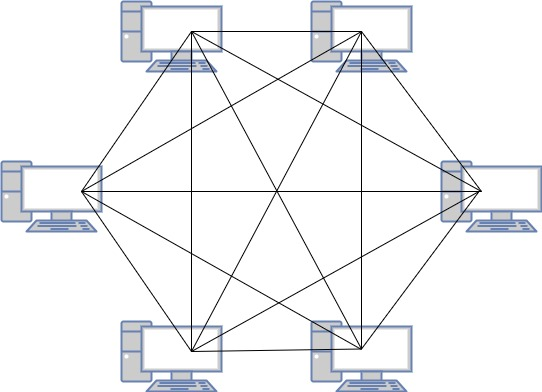
\includegraphics[width=0.3\textwidth]{Images/P2P.jpg}
	\caption{Sieć typu P2P}
	\label{fig:P2P}
\end{figure}
\newline Każdy z komputerów połączonych do takiej sieci zawierałyby swoją własną kopię danych, dzięki czemu przy utracie danych na którymś z komputerów, można je odzyskać poprzez pobranie ich od innego użytkownika.
Istnieje również alternatywne rozwiązanie tego założenia, mianowicie przechowywanie danych na różnych serwerach, co widać w przykładzie zobrazowanym przez \figurename{~\ref{fig:SiecSerwery}}. Jest to w obecnych czasach częściej spotykane rozwiązanie, lecz nie spełnia ono kolejnej potrzeby, która jest opisana w następnej sekcji.
\begin{figure}[!ht]
	\centering
		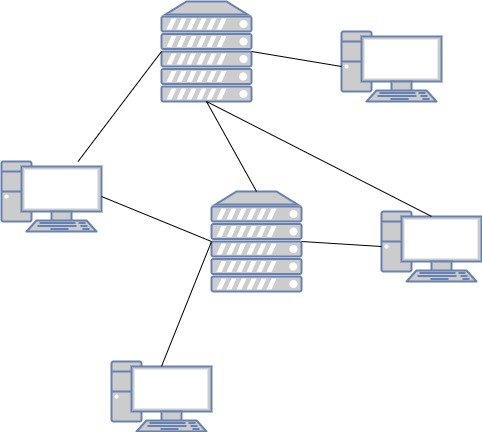
\includegraphics[width=0.3\textwidth]{Images/Siec_serwery.jpg}
	\caption{Sieć z różnymi serwerami}
	\label{fig:SiecSerwery}
\end{figure}
\newline

\subsection{Decentralizacja}
\label{ssec:Decentralizacja}
Kolejnym wymogiem, jaki powinien być zrealizowany w naszej pracy, jest wykonanie aplikacji, która będzie działać w sposób zdecentralizowany. Oznacza to, że żaden użytkownik nie może mieć kontroli nad innymi, a co za tym idzie, nie ma żadnej scentralizowanej jednostki, która może zarządzać przepływem danych w sieci. Z tego powodu drugie rozwiązanie, które zostało wspomniane w poprzedniej sekcji, czyli wykorzystanie różnych serwerów do przechowywania danych, nie może zostać wykorzystane w naszej implementacji. Wynika to z faktu, iż osoby zarządzające serwerami mogą arbitralnie zablokować niepożądanym w ich ocenie osobom dostęp do zasobów danych.

\section{Przypadki użycia}
\label{sec:PrzypadkiUzycia}
\begin{figure}[!ht]
	\centering
		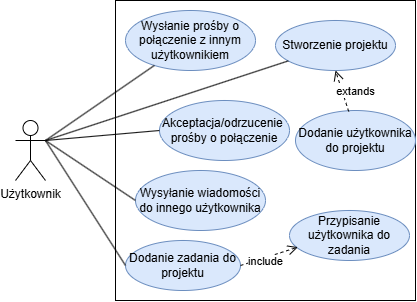
\includegraphics[width=0.5\textwidth]{Images/PrzypadkiUzycia.png}
	\caption{Diagram przypadków użycia}
	\label{fig:PrzypadkiUzycia}
\end{figure}
Opis przypadków użycia na podstawie diagramu, który pokazuje \figurename{~\ref{fig:PrzypadkiUzycia}}:
\begin{itemize}
\item {Wysłanie prośby o połączenie z innym użytkownikiem} - Użytkownik podaje adres ip i port innego użytkownika i wysyła do niego prośbę o połączenie. Jeśli drugi użytkownik zaakceptuje, zostanie nawiązane połączenie i zostanie dodany do listy połączonych użytkowników.
\item {Akceptacja/Odrzucenie prośby o połączenie} - Użytkownik po otrzymaniu prośby o połączenie może ją zaakceptować bądź odrzucić.
\item {Wysłanie wiadomości} - Użytkownik wysyła wiadomość tekstową do drugiego użytkownika z którym jest połączony.
\item {Stworzenie projektu} - Użytkownik tworzy projekt do którego jest automatycznie dodany. Podczas tworzenia projektu użytkownik nadaje mu nazwę i ma możliwość dodania do niego innych użytkowników (przypadek dodanie użytkownika do projektu).
\item {Dodanie użytkownika do projektu} - Podczas tworzenia projektu użytkownik może dodać do niego innych, połączonych z nim, użytkowników wybierając ich z listy.
\item {Dodanie zadania do projektu} - Użytkownik ma możliwość dodania zadania do danego projektu. Użytkownik podaje: nazwę zadania, przypisanych użytkowników(przypadek Przypisanie użytkownika do zadania), priorytet, termin wykonania, oznaczenia.
\item {Przypisanie użytkownika do zadania} - Podczas dodawania zadania do projektu(przypadek Dodanie zadania do projektu) użytkownik musi przypisać co najmniej jednego użytkownika przypisanego do danego projektu (z listy).
\end{itemize}

\section{Logika biznesowa}
\label{sec:LogikaBiznesowa}
Należy na początku poświęcić kilka słów wyjaśnienia, co kryje się pod pojęciem logika biznesowa. Jest to warstwa aplikacji odpowiedzialna za wykonywanie funkcji, które umożliwiają jej prawidłowe oraz spójne działanie. Kontroluje ona, co użytkownik może wykonać w aplikacji oraz definiuje warunki, jakie muszą zajść, by do danej czynności doszło. Przykładowo użytkownik może w programie definiować nowe zadanie, lecz jest to obarczone konkretnymi warunkami, takimi jak: 
\begin{itemize}
    \item projekt, w którym chce je dodać, musi istnieć,
    \item użytkownik musi mieć do dostęp do tego projektu,
    \item musi uzupełnić szczegóły dotyczące nowego zadania jak chociażby nazwa zadania czy też jaka osoba jest do niego przypisana.
\end{itemize}
Niespełnienie któregokolwiek z warunków sprawia, że nie może zostać utworzone nowe zadanie. Logika biznesowa nie zajmuje się wyłącznie tym, gdyż wykonywane są w niej również wspomniane na początku rozdziału algorytmy. Implementacja ich w tym miejscu związana jest z co najmniej z dwoma potrzebami, które należy spełnić w naszym programie, mianowicie są to:
\begin{itemize}
    \item możliwie jak najkrótszy czas dostępu do danych,
    \item responsywność interfejsu graficznego.
\end{itemize}
Dostęp do danych powinien jak najwierniej odwzorowywać operacje atomowe na mikroprocesorze, tak aby był on możliwie najkrótszy. To sprawia, że gdy przykładowo inny użytkownik będzie chciał pobrać od nas jakieś informacje, to żeby nie musiał oczekiwać na zwolnienie zasobu, który jest wykorzystywany do wyliczania wyniku algorytmu. W warunkach, w których przeważnie testowaliśmy nasz program, czyli uruchomionych kilka klientów, nie byłoby odczuwalnej różnicy w czasie dostępu, natomiast jeśli przełożyć tę różnicę na chociażby kilkaset klientów, to każda próba pobrania od innych użytkowników danych wiązałaby się ze zwiększonym opóźnieniem. Podobnie jak do czasu dostępu rzecz ma się z responsywnością interfejsu, gdyż gdyby on musiał wykonywać obliczenia związane z algorytmami, to użytkownik mógłby odczuć, jakby program co chwila nie odpowiadał.
%--TODO--

\subsection{Komunikacja między użytkownikami}
\label{ssec:Komunikacja}
Jednym z istotnych elementów naszego programu jest możliwość komunikowania się ze sobą użytkowników. W tym celu wykorzystaliśmy porozumiewanie się za pomocą protokołu HTTP. Wynika to z następujących zapotrzebowań:
\begin{itemize}
    \item bezpośrednia komunikacja między użytkownikami,
    \item dostosowanie przesyłanych danych w zależności od kontekstu,
    \item prostota zastosowania danego protokołu,
    \item szeroko dostępna dokumentacja protokołu.
\end{itemize}
Alternatywą do HTTP jest IPFS - InterPlanetary File System, który na pierwszy rzut oka wygląda na  lepsze rozwiązanie do naszej pracy, gdyż w przeciwieństwie do HTTP jest przystosowany do pracy w sieci rozproszonej, czym jest głównie reklamowany \cite{IPFS}. Nie wybraliśmy go jednak w naszej pracy ze względu na wcześniejsze doświadczenie z protokołem HTTP w poprzednich naszych projektach oraz na znikomą ilość pomocy dydaktycznej związanej z wykorzystaniem go w aplikacjach. Problemem z IPFS jest również to, że jego przystosowanie do sieci rozproszonej tyczy się treści przesyłanych przez ten protokół, aniżeli komunikacji między osobami. Jest to dobre rozwiązanie w przypadku, gdyby nasza aplikacja polegała wyłącznie na przechowywaniu danych i przesyłaniu ich między użytkownikami. Ze względu na zastosowanie łańcucha bloków, o którym można więcej przeczytać w sekcji \nameref{sec:Blockchain}, w którym zapisywanie danych nie odbywa się natychmiast, nie jest to koniecznie dobre rozwiązanie.
\clearpage
\begin{figure}[!ht]
    \centering
		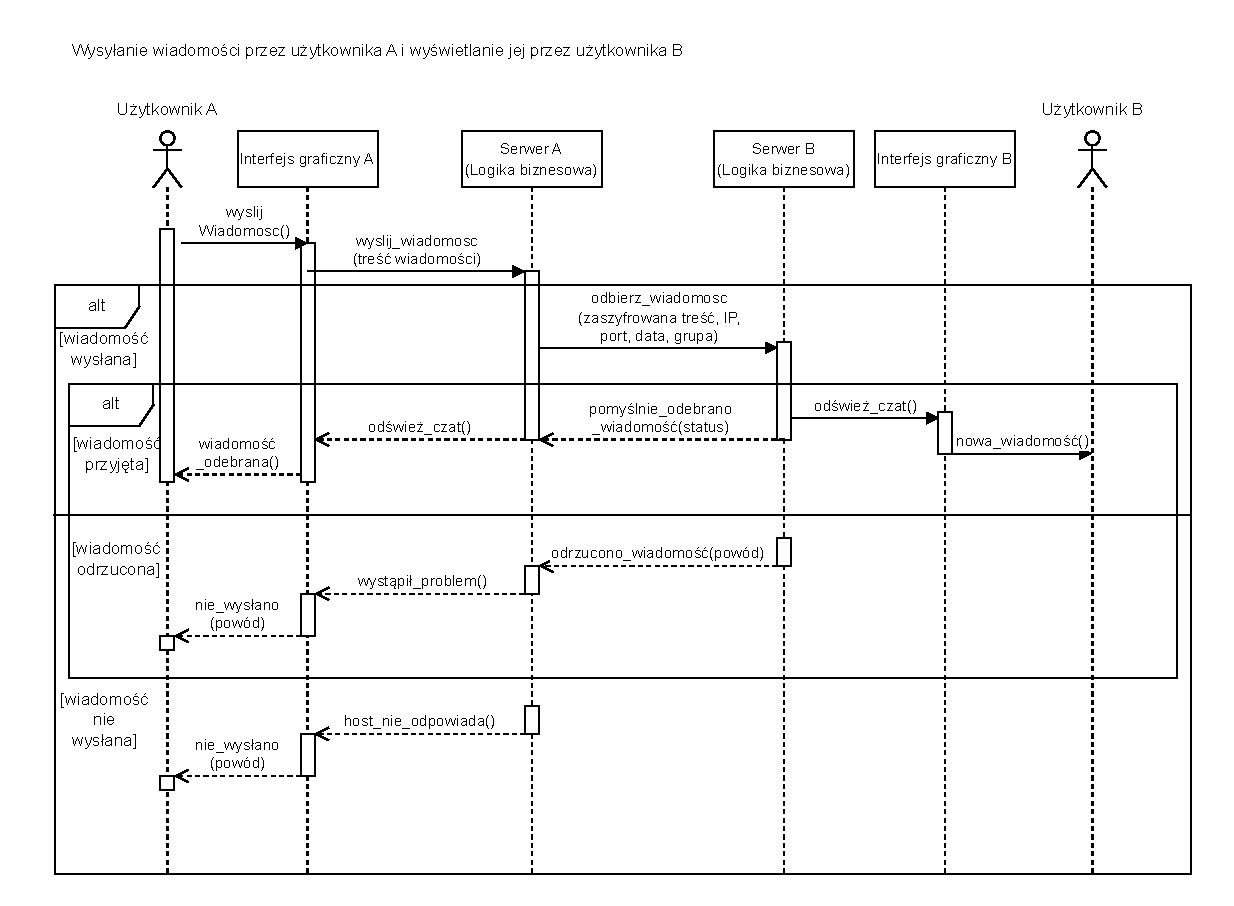
\includegraphics[width=1\linewidth]{Images/wysylanie_wiadomosci.pdf}
	\caption{Diagram sekwencji wysłania wiadomości i jej wyświetlenia}
	\label{fig:wysylanieWiadomosci}
\end{figure}
\par Po przedstawieniu cech protokołu HTTP i uzasadnieniu jego wyboru, pora przejść do omówienia tego, jak on jest w praktyce wykorzystywany w naszej pracy. Komunikacja po tym protokole dostępna jest za sprawą uruchamianego w naszym programie serwera. Odpowiedzialna jest za to biblioteka dostępna w języku Python - \textit{Flask}. Umożliwia on otrzymywanie danych od innych użytkowników jak również odsyłanie im odpowiedzi wraz z żądanymi informacjami. Diagram sekwencji przedstawiony w \figurename{ \ref{fig:wysylanieWiadomosci}} posłuży tutaj jako ilustracja przykładu takiej komunikacji. Sytuacja na tym diagramie jest następująca: Użytkownik A pragnie wysłać wiadomość do Użytkownika B, a ten chce wyświetlić jej treść. W celu uproszczenia diagramu zakładamy, że obaj użytkownicy mają otwarty czat ze sobą, zatem interfejs graficzny nie przesyła informacji, jakiego czatu dotyczą dane wiadomości. Na początek Użytkownik A wypełnia w interfejsie graficznym aplikacji pole wiadomości jej treścią i zleca programowi jej wysłanie. Warstwa prezentacji przesyła odpowiednie informacje do logiki biznesowej aplikacji, tj. treść wiadomości. Następnie logika biznesowa w ramach bezpieczeństwa szyfruje wiadomość kluczem prywatnym Użytkownika A. W tym momencie następuje komunikacja między użytkownikami za pomocą protokołu HTTP, gdyż logika biznesowa zleca serwerowi, uruchomionemu w oddzielnym wątku, wysłanie zapytania HTTP do serwera Użytkownika B pod odpowiedni adres. Struktura adresu jest następująca: 
\textit{http://<Adres~IP>:<Numer~portu>/<funkcja\_do\_wywolania>}
W tym konkretnym przypadku przedstawionym na diagramie, w naszym projekcie byłby to adres: \textit{http://<Adres~IP>:<Numer~portu>/receive\_message}.
Wysłanie żądania odbywa się za pomocą gotowej funkcji przygotowanej w bibliotece \textit{Flask}, odpowiedzialnej za działanie serwera (funkcja \textit{requests.post()}). Wszelkie dane, które mają trafić do drugiej osoby, zapisywane są w formacie JSON. Po wysłaniu zapytania HTTP, serwer Użytkownika B odbiera je i przekazuje dalej do logiki biznesowej. W przypadku, gdy Użytkownik B otrzymał prawidłową wiadomość, wysyła odpowiedź HTTP ze statusem sukcesu, oznaczającym wysłanie prawidłowego żądania. Jeśli jednak z jakiegoś powodu Użytkownik A wysłał błędną wiadomość, np. została źle sformatowana, bądź Użytkownik B posiada przestarzały klucz publiczny wysyłającego, przez co nie mógł jej prawidłowo odszyfrować, to wysyła odpowiedź ze statusem błędu. Użytkownik A w zależności od tego, jaką otrzymał odpowiedź, wykonuje odpowiednią czynność. Dodaje on do swojej puli wiadomości tę wysłaną do Użytkownika B tylko wtedy, gdy się okaże, że została ona prawidłowo odebrana. Zostało to również odzwierciedlone na analizowanym diagramie.

\subsection{Metodologia "Załatwianie Spraw"}
\label{ssec:GTD}
Istotną rzeczą według której kierowaliśmy się w implementacji modułu planera w logice biznesowej jest metodologia "Załatwianie Spraw" \ang{Getting Things Done} (stąd skrót GTD). Jest ona autorstwa Davida Allena, którą po raz pierwszy przedstawił światu w swojej książce o tym samym tytule \cite{GTD}. Polega ona na odpowiednim planowaniu swoich zadań w taki sposób, by osoba, która wdraża GTD, myślała jedynie o tym, w jaki sposób realizować te zadania, bez potrzeby zapamiętywania ich. Po ich zaplanowaniu, użytkownik nie powinien już myśleć o tych zadaniach do momentu, gdy zasięgnie do planera. Aby zrozumieć istotę tej metodologii, należy wymienić pięć kluczowych punktów, jakie należy spełnić używając jej. Głównymi czynnościami jakie należy wykonać to:
\begin{itemize}
    \item Gromadzenie - zbieranie do jednego miejsca wszystkich planów, zadań, pomysłów z jakimi w ostatnim czasie miała styczność dana osoba,
    \item Analiza - podejmowanie po kolei decyzji na temat poszczególnych zadań. Są to decyzje pokroju:
    \begin{itemize}
        \item czy ono może zostać wykonane natychmiast,
        \item czy z tym zadaniem są związane inne zadania,
        \item czy to zadanie jest do wykonania przeze mnie. 
    \end{itemize}
    \item Porządkowanie - przypisywanie cech oraz kontekstu poszczególnym zadaniom. W tym punkcie należy przypisać do nich to, gdzie mają zostać wykonane, np. w domu, w biurze, w jaki sposób należy je zrobić, np. przez telefon, na miejscu,
    \item Przegląd - etap w którym użytkownik powinien się upewnić, czy w prawidłowy sposób uporządkował zadania w poprzednich punktach,
    \item Realizacja - poświęcenie swojej uwagi na wykonywaniu zadań zapisanych w poprzednich etapach, respektując ich cechy oraz kontekst, tj. zadania do wykonania w biurze powinny być wykonane właśnie tam.
\end{itemize}
W implementowanym systemie stworzony został moduł planera, który pozwala realizować zadania na podstawie dostosowanej do warunków technicznych, w jakich użytkownicy mogą go wykorzystywać. Z tego względu etapy dotyczące gromadzenia, analizy i porządkowania zostały ujednolicone w jeden wspólny punkt. W ten sposób został uproszczony proces dodawania nowych zadań przez użytkownika. To sprawia, że jest on również bardziej wydajny.

\section{Przechowywanie danych}
\label{sec:PrzechowywanieDanych}
Trzecią z warstw aplikacji, jakie można wyodrębnić zaraz po warstwie prezentacji (interfejsu graficznego) oraz logiki biznesowej, jest warstwa przechowywania danych. Jest ona odpowiedzialna za dostęp do danych używanych w trakcie korzystania aplikacji. Warstwa ta ma gwarantować to, że w możliwie jak najkrótszym czasie uzyska się żądane dane oraz ich zapis przebiegnie bez najmniejszych zakłóceń. W przypadku awarii systemu i utraty danych z tego tytułu, warstwa ta powinna być w stanie odtworzyć je na podstawie ich kopii, które znajdują się na komputerach innych użytkowników. Proces ten powinien przebiegać na tyle sprawnie, żeby użytkownik mógł nawet nie zwrócić uwagi na fakt, że przez krótki czas mógł mieć błędne dane.
%TODO

\subsection{Łańcuch bloków}
\label{sec:Blockchain}
Użycie sieci P2P w naszej pracy sprzyja temu, by skorzystać ze struktury danych, która jest przystosowana do takiego rozwiązania. Jedną z takich struktur jest łańcuch bloków \ang{Blockchain}. Jest to jednokierunkowa lista, w której nowe rekordy, zwane blokiem, są przyłączane zawsze na jej końcu. Każdy z tych bloków jest odpowiednio przywiązany do ich sąsiadów. Jest to możliwe dzięki zastosowaniu odpowiednio zaszyfrowanego skrótu z treści \ang{Hash} poprzedzającego go bloku. Przywiązanie te najprościej będzie przedstawić na podstawie naszego kodu, widocznego w \lstlistingname{~\ref{lst:PolaBlock}}, w którym zawarte są pola, jakie zawiera obiekt klasy Block.
\begin{lstlisting}[language=Python, extendedchars=true, caption={Pola obiektu klasy Block}, label={lst:PolaBlock}]
self.index
self.data
self.digitalEncryption
self.hostVerifier
self.portVerifier
self.publicKeyVerifier
self.lastDigitalEncryption
\end{lstlisting}
Pola tej klasy służące do łączenia ze sobą bloków to \textit{digitalEncryption} oraz \textit{lastDigitalEncryption}, z czego to pierwsze informuje o skrócie z treści aktualnego bloku, a drugie z bloku poprzedzającego. Przy tworzeniu łańcucha bloków należy stworzyć również blok "zerowy". Wynika to z faktu, że pierwszy blok, który rozpoczyna łańcuch, nie posiada swojego poprzednika, zatem pole \textit{lastDigitalEncryption} musi mieć ustawioną specjalną wartość. W różnych implementacjach łańcucha bloków, jakie napotkaliśmy w publicznych repozytoriach kodów jak np. \url{https://github.com} najczęściej spotykaliśmy rozwiązanie, że skrót treści "zerowego" bloku był przepisywany do pola z  wartością poprzednika. Z takiego pomysłu również skorzystaliśmy w naszej implementacji łańcucha bloków, którą bazujemy na implementacji znajdującej się w repozytorium pod linkiem: \url{https://github.com/breqdev/blockchat} (Dostęp: 2024-12-07). Poza tymi dwoma polami, warto zwrócić uwagę również na pozostałe. Pole \textit{index} umożliwia pozycjonowanie bloków w całym łańcuchu, natomiast pole \textit{data} jest tym kluczowym, gdyż właśnie w nim zapisywane są wszelkie dane odnośnie grupy wiadomości czy informacji na temat sfinalizowanego projektu z modułu planera. Grupa wiadomości to nic innego jak zbiór \textit{x} wiadomości przesłanych między użytkownikami, gdzie \textit{x} oznacza ich liczbę. Domyślnie jest to wartość 20. Pola \textit{hostVerifier}, \textit{portVerifier} oraz \textit{publicKeyVerifier} są związane ze szyfrowaniem bloku przez podpis odpowiedniego sygnatariusza, czyli osoby wybranej w PoS do zweryfikowania autentyczności otrzymanych danych. Te pola to odpowiednio: adres IP, numer portu oraz klucz publiczny tego użytkownika. Więcej informacji odnośnie roli tej osoby przy szyfrowaniu bloku znajduje się w rozdziale \nameref{ssec:KonsensusUzycie}. Po przedstawieniu zasad działania łańcucha bloków oraz omówieniu tego jak wygląda on w naszym programie, pora na uzasadnienie wyboru akurat tego rozwiązania.
\chapter{Podsumowanie}
Udało się nam zrealizować wszystkie stawiane systemowi wymagania:
\begin{itemize}
    \item System działa w architekturze rozproszonej, każdy z użytkowników jest równy innym, system został zaimplementowany bez użycia głównego serwera, co pozwoliło uniknąć centralizacji
    \item W systemie można wysyłać wiadomości do innych użytkowników
    \item W systemie można tworzyć grupy z dowolnymi użytkownikami i treść wiadomości dla osób z poza grupy nie jest dostępna
    \item System oparty jest o mechanizmy działające w kryptowalutach mające na celu zapewnienie w nim uczciwości i bezpieczestwa
    \item System posiada graficzny interfejs użytkownika, pozwalający na łatwiejsze korzystanie z niego
    \item System posiada szyfrowanie danych w celu zapewnienia poufności i tego, aby nikt z poza sieci nie mógł odczytać treści wiadmości
    \item W systemie zapewniona jest niezaprzeczalność wiadomości poprzez ich podpisywanie podpisem cyfrowym przez weryfiktora
    \item W systemie zaimplementowane są mechanizmy zapwenianiania uczciwości poprzez implementację algorytmów osiągania konsensusu
    \item W systemie można planować zadania do wykonania
\end{itemize}
\vspace{0.3\baselineskip}
Podsumowując stworzyliśmy działający system z w pełni działającym graficznym interfejsem użytkownika, który pozwala na komunikację między użytkownikami i jak i tworzenie dowolnie dużych grup użytkowników, dla których odbywa się komunikacja grupowa. W systemie zapewniona jest poufność poprzez zastosowanie szyfrowania wiadmości, niezaprzeczalność przez podpisywanie cyfrowe bloków wiadomości i mechanizmy zapewniania uczciwości systemu przez algorytmu osiągania konsensusu.

% bibliografia
% ieeetr - etykiety numerowane w kolejności wystąpienia w tekście
\bibliographystyle{ieeetr}
\bibliography{Chapters/Bibliography}

% wykazy 
\listoffigures
\listoftables
\listofequations

% dodatki
\appendix
% słaba funkcja
% \titlecontents{chapter}[0cm]{}{\normalsize\bfseries{\appendixname\space}\contentslabel{-1pt}\hspace*{0.6cm}}{}{\titlerule*[4.5pt]{.}\hspace*{5pt}\contentspage}

\chapter*{Dodatek A: Uzupełnienie wymogów}
\addcontentsline{toc}{chapter}{Dodatek A}
% Póki co jest problem ze słowem dodatek w spisie treści. Funkcja wklejona na początku działa słabo. Powyższe linijki obchodzą ten problem bardzo dobrze, ale dodatki trzeba sobie numerować "ręcznie"

No i mamy jeszcze dodatek - jeśli trzeba

Dodatki należy oznaczać kolejnymi dużymi literami alfabetu. W dodatkach należy umieszczać elementy uzupełniające, które powinny zostać dołączone do pracy, np. w celu prezentacji wykonanych obliczeń, schematy ideowe.  
\end{document}
